\chapter{System characterization and Preliminary Results}
In this chapter I present the results of the studies in the vertical plane of the piezo-movers calibration factor per block, the BPM signal calibration per BPM and the dynamic range measurement for the IPB system. The resolution is estimated by the analysis of the electronics noise limit and the beam trajectory reconstruction from jitter acquisitions. The system is also used to test feedback in one BPM.\par
Finally the status of the BPM system is shown with remarks about the ongoing work to improve the current performance.\par
\section{Calibration}\label{s:cals}
The calibration factor is obtained per cavity and in the vertical plane $y$ by measuring the position signal change as a function of the physical displacement of the cavity. Two factors are used to obtain each calibration : the movers' displacement versus voltage setting $C_m$ [$\mu$m/V] and the cavity response versus voltage setting $C_c$ [a.u./V]. Therefore the cavity calibration factor is $C_{bpm}=C_c/C_m$ [a.u./$\mu$m].\par
\subsection{Movers' Calibrations $C_m$}\label{s:calcm}
Prior to installation, the movers' displacement versus voltage setting was measured per BPM block. An interferometer with better than 1 nm resolution was used to measure the BPM vertical position as shown in Fig.~\ref{f:interfero}. As the head is located on top of the BPM, positive displacement implies negative change in the intereferometer readout. Four cycles are shown in Fig. \ref{f:fourcycles}, two descending and two rising, covering the total dynamic range and divided in 100 steps, with a 3~s settling time between steps.\par
\begin{figure}[!htb]
\centering
\begin{subfigure}[b]{0.9\textwidth}
\centering
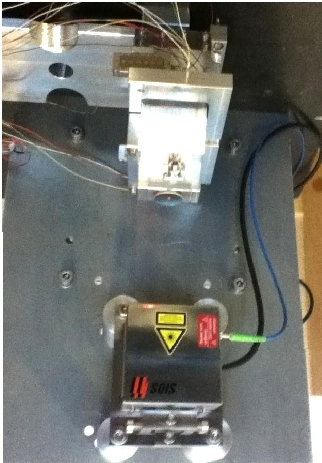
\includegraphics[scale=0.6,angle=180]{interfero.jpg}\caption{Picture of SIOS interferometer used to test the movers. Precision is better than 1 nm.}\label{f:interfero}
\end{subfigure}\\%\hspace*{1cm}\\
\begin{subfigure}[b]{0.9\textwidth}
\centering
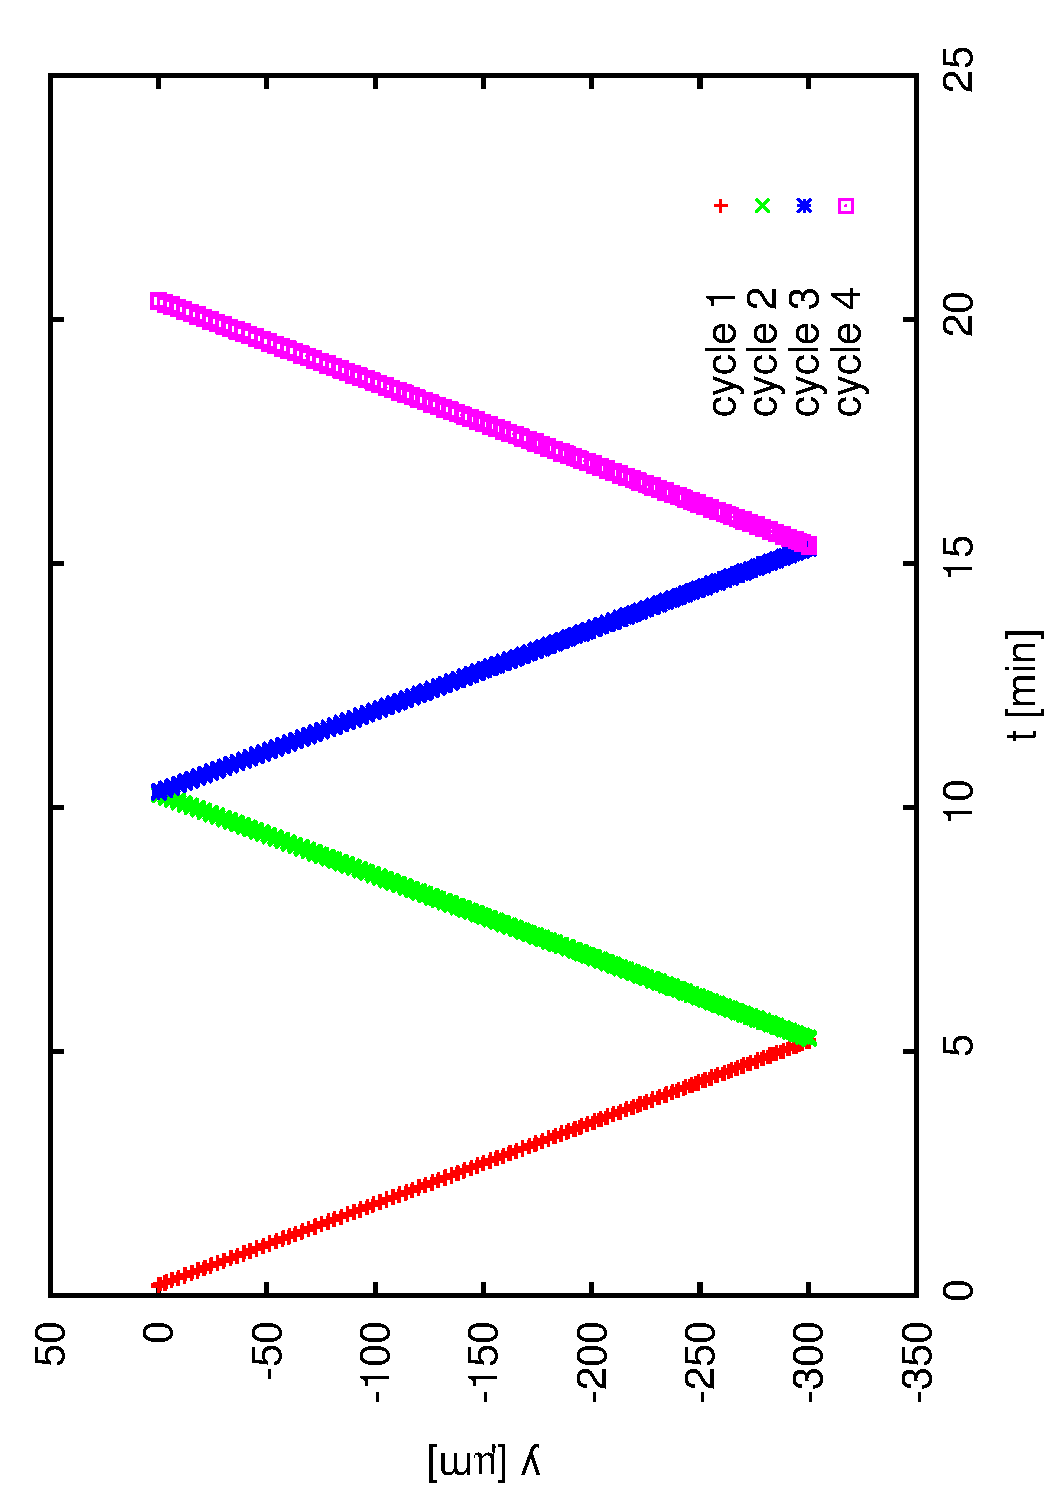
\includegraphics[scale=0.32,angle=-90]{image01.pdf}\caption{Four cycles are performed over the entire dynamic range of movers.}\label{f:fourcycles}
\end{subfigure}\caption{Movers calibration test setup for the vertical plane.}\label{f:cmtest}
\end{figure}
\subsubsection{Block AB movers, Cedrat}
Linearity was tested in the four cycles with feedback. Fig. \ref{f:Cedratmsteps} shows the mover step and Fig. \ref{f:Cedratlinres} shows the residuals from the linear fitting substraction on each cycle.\par
\begin{figure}[!htb]
 \centering\hspace*{-0.6cm}
\begin{subfigure}{0.4\textwidth}
 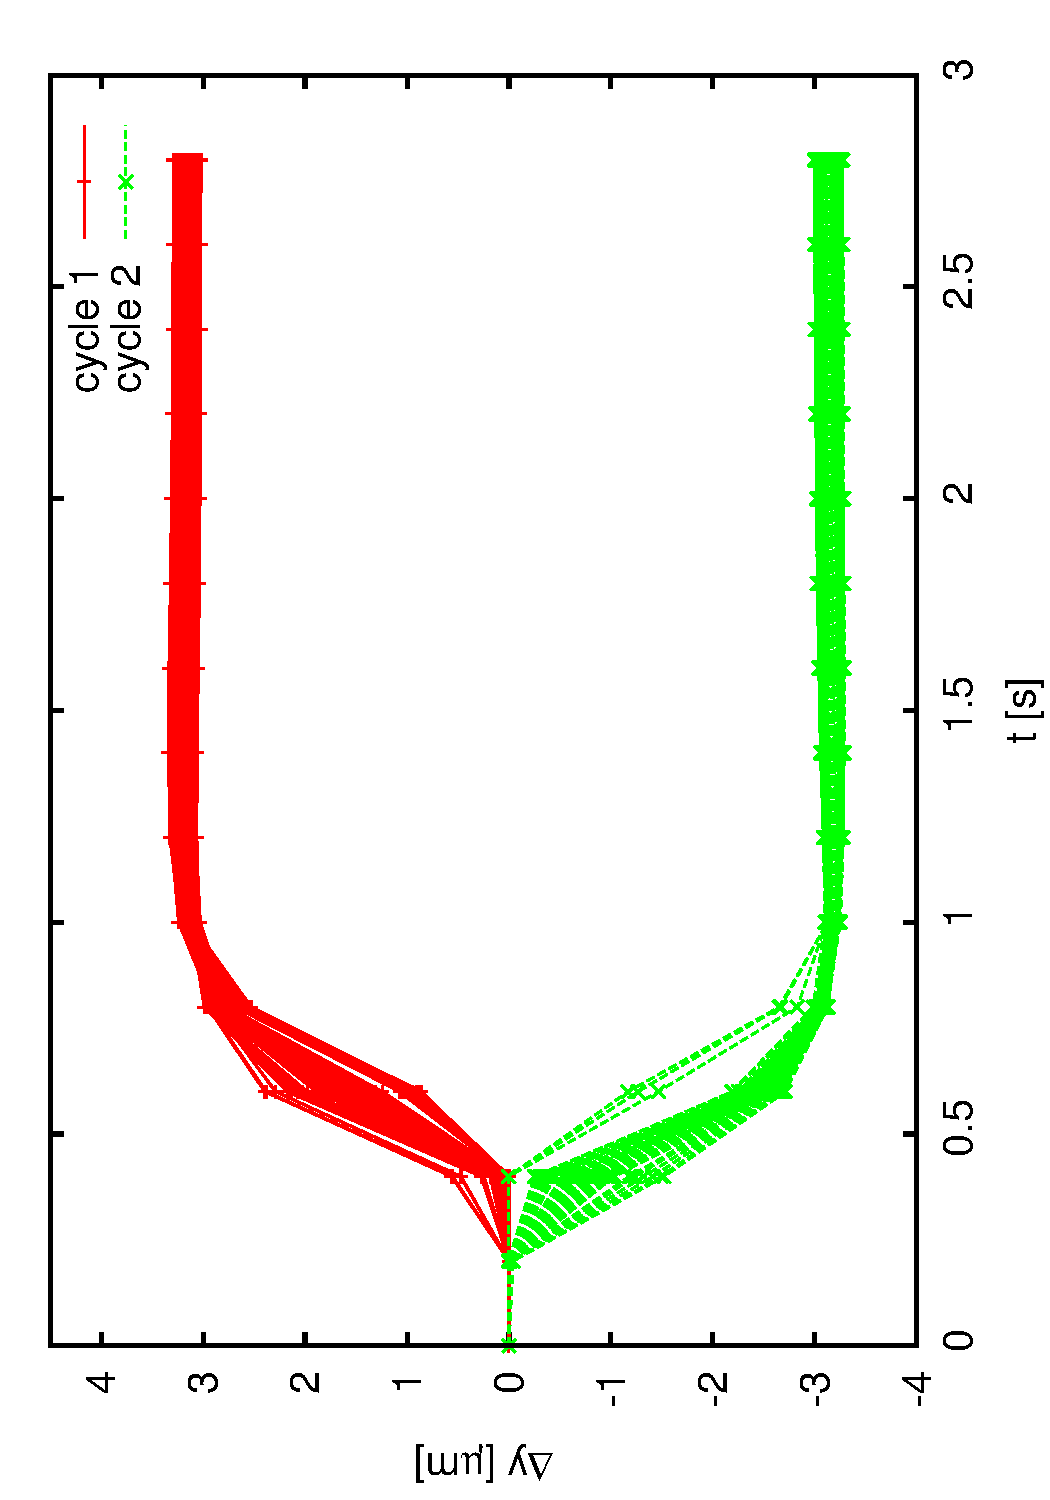
\includegraphics[angle=-90,scale=0.30]{image24.pdf}\caption{Settling speed with feedback for Cedrat movers.}\label{f:Cedratmsteps}
\end{subfigure}\hspace*{1.5cm}
\begin{subfigure}{0.4\textwidth}
 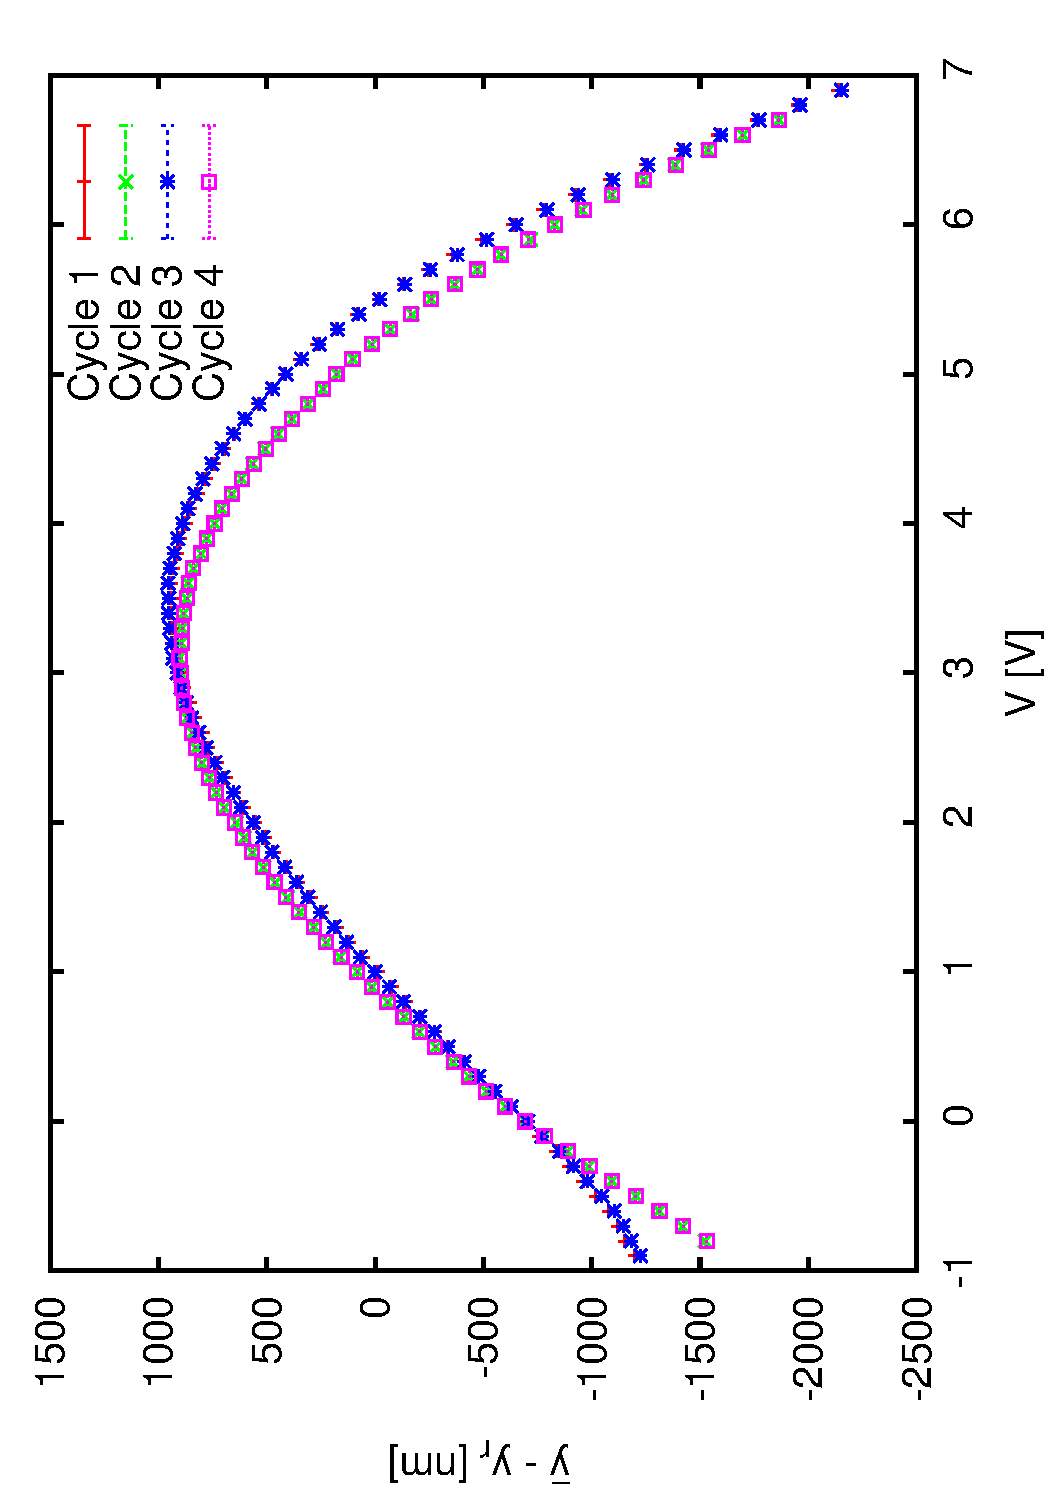
\includegraphics[angle=-90,scale=0.30]{image26e.pdf}\caption{Residual non-linearity (with fb), after substraction of linear fitting on cedrat movers.}\label{f:Cedratlinres}
\end{subfigure}\caption{Block AB movers, linearity test over four cycles.}\label{f:Cedratfeedback}
\end{figure}
The calibration mean from these 4~cycles is $C_{mAB} = (-31.015\pm12)\mu$m/V. This value is valid for ranges were the residual is constant enough, therefore, it is recommended to use the movers with voltage settings in the middle of the total dynamic range and to scan over less than 1~V. Improved calibration over full the range can be obtained using a non-linear function.\par
The step stability was tested by moving back and forth the voltage setting hundreds of times. Figure \ref{f:Cedratstepstab} shows that 10~nm steps are observable and Fig. \ref{f:Cedratstab} shows 1.1~nm of stability on each setting.\par
\begin{figure}[!htb]
 \centering\hspace*{-0.6cm}
\begin{subfigure}{0.4\textwidth}
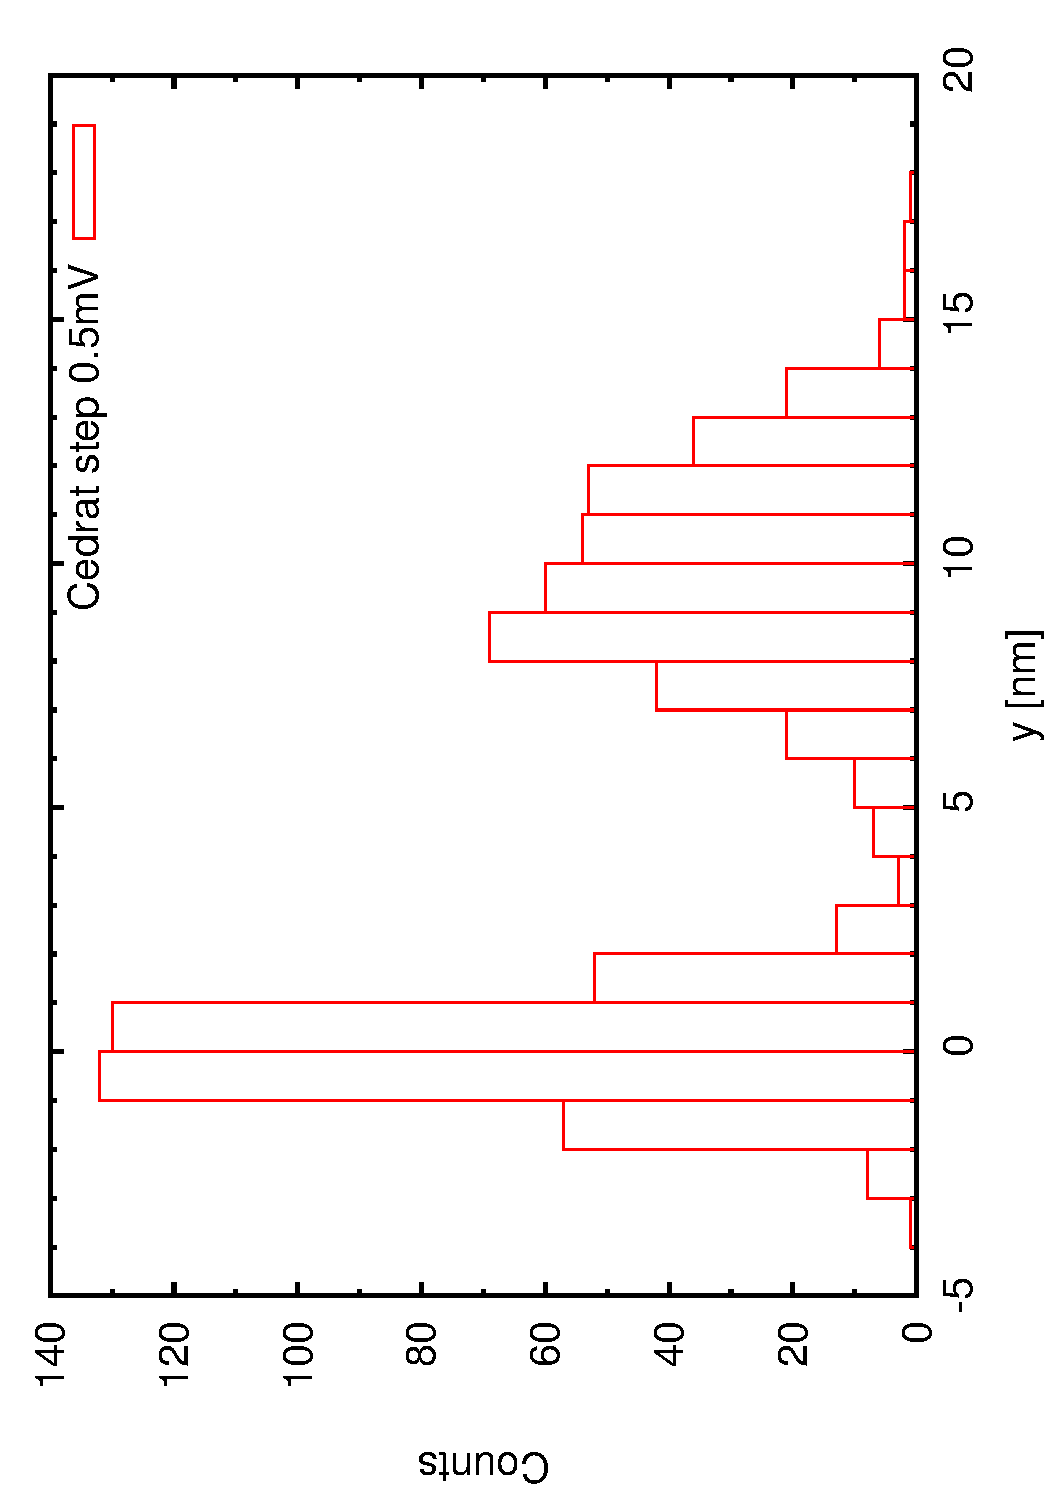
\includegraphics[angle=-90,scale=0.30]{imagestep12a.pdf}\caption{Minimum voltage setting variation back and forth tested was 0.5 mV.}\label{f:Cedratstepstab}
\end{subfigure}\hspace*{1.5cm}
\begin{subfigure}{0.4\textwidth}
 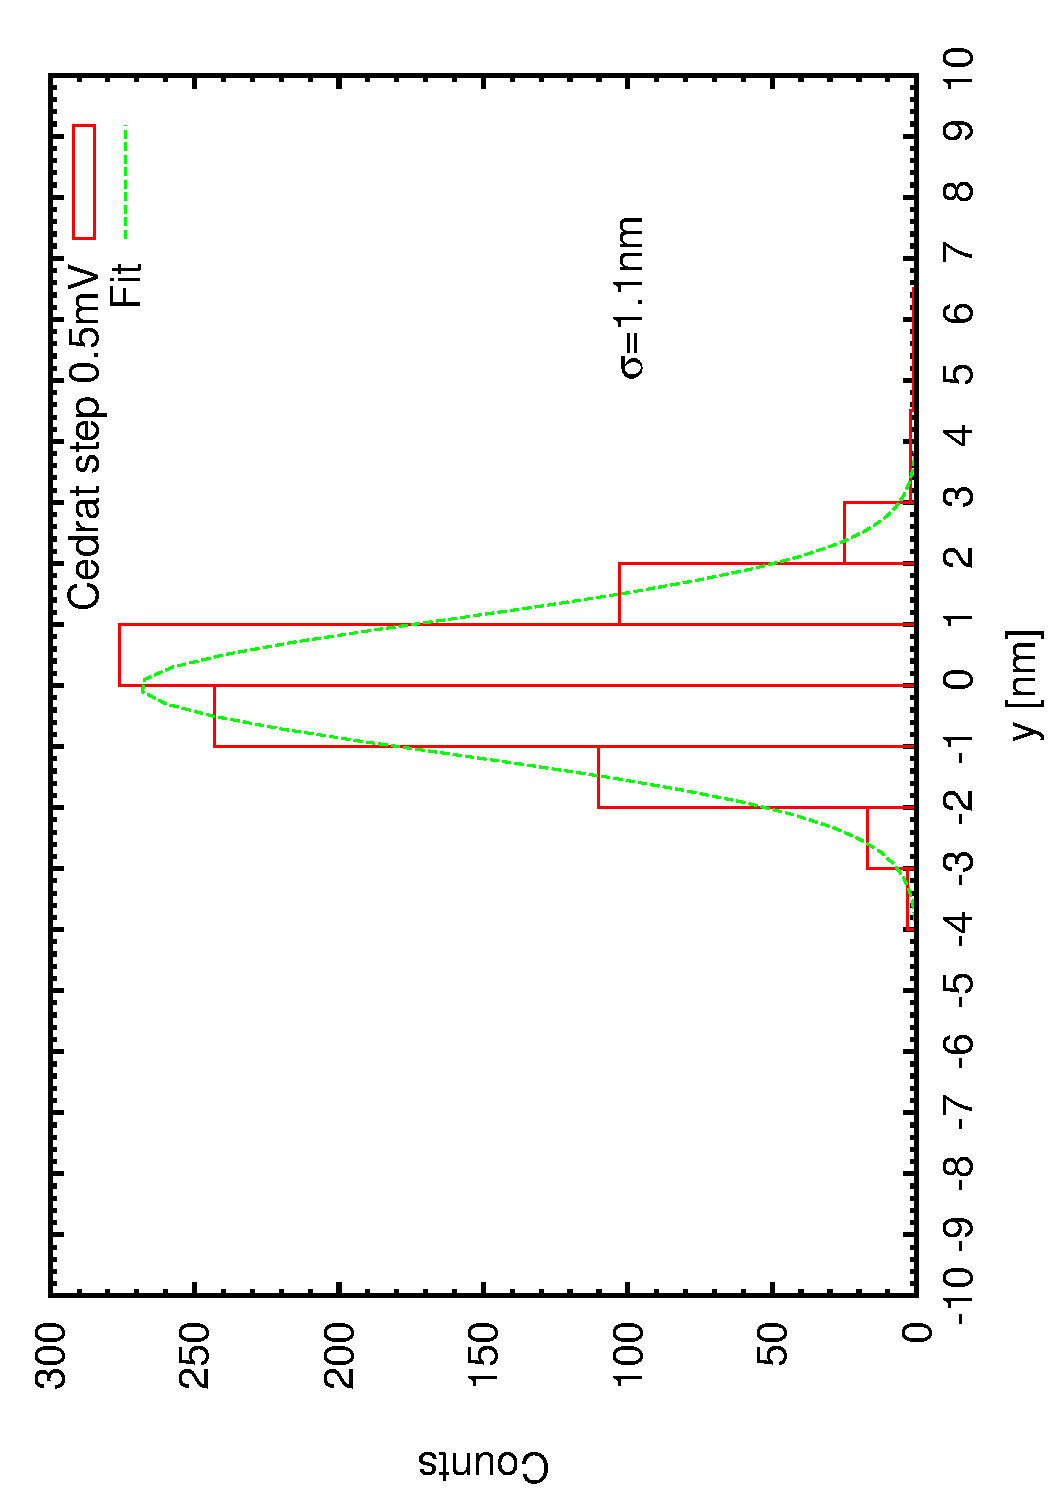
\includegraphics[angle=-90,scale=0.30]{imagestep12.pdf}\caption{Stability at fixed voltage setting.}\label{f:Cedratstab}
\end{subfigure}\caption{Block AB movers minimum step and stability.}\label{f:Cedratstability}
\end{figure}
Coupling effect of horizontal displacement on the vertical plane was also tested. Figure \ref{f:Cedratcoupling} shows a vertical position variation of 2.5 $\mu$m (1\%) over the full horizontal dynamic range.\par
\begin{figure}[!htb]
\centering
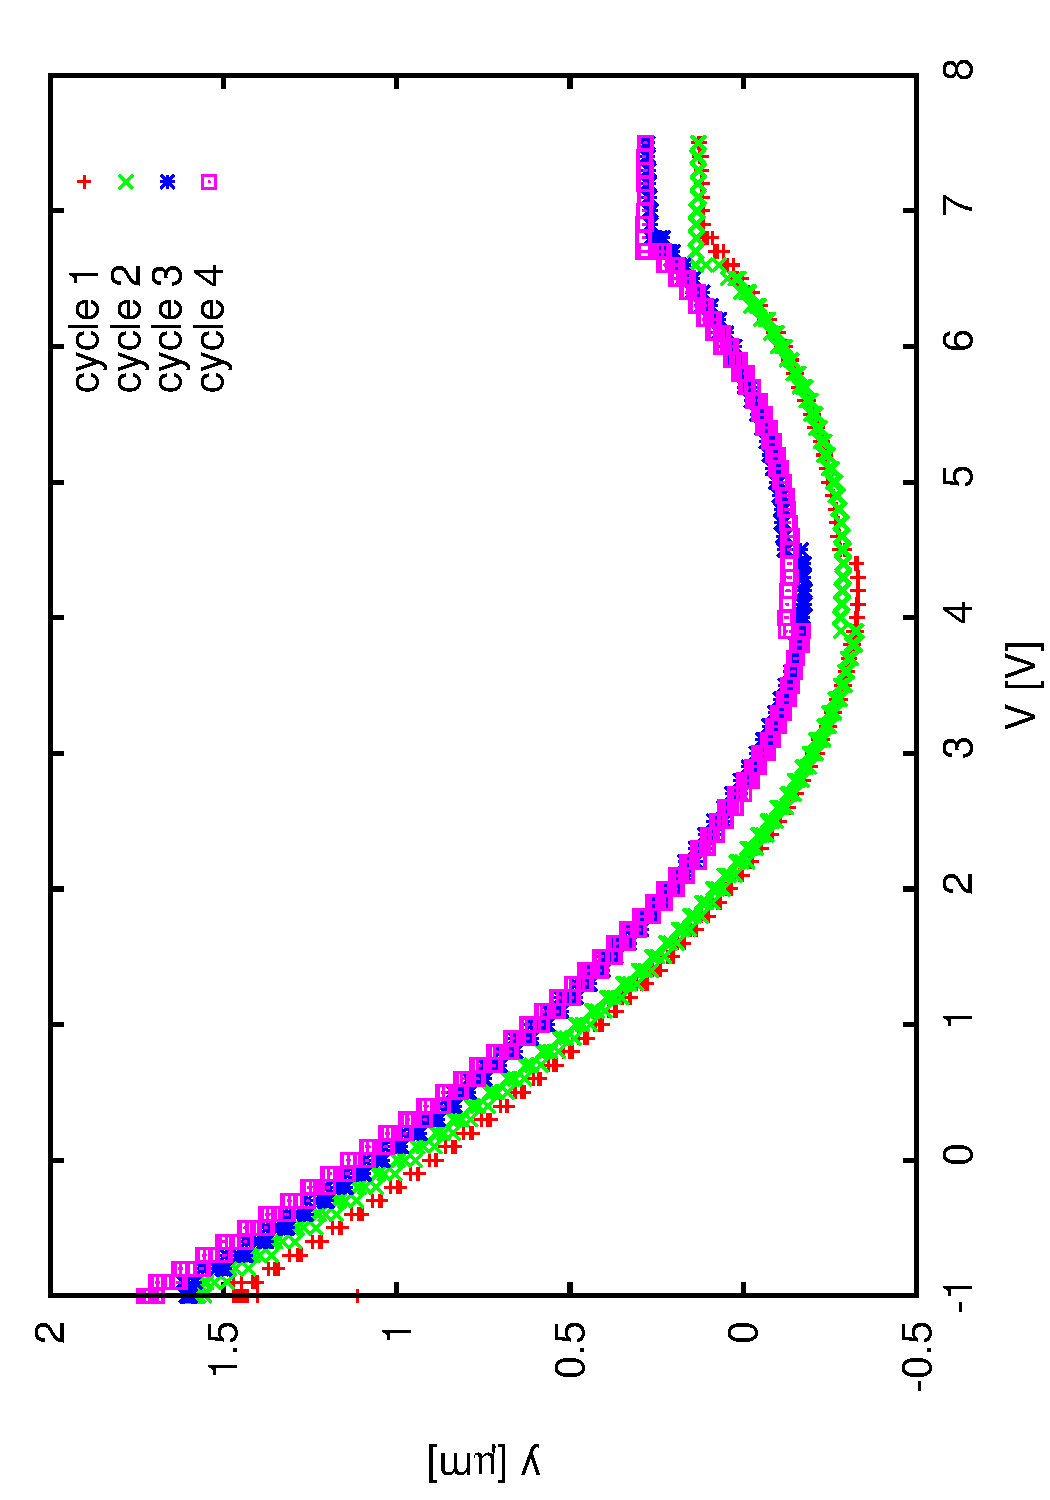
\includegraphics[scale=0.32,angle=-90]{image62.pdf}\caption{Horizontal to vertical coupling of movers motion.}\label{f:Cedratcoupling}
\end{figure}
Only the readbacks from the control box are available after installation indicating current mover position. Results from readback linearity with respect to voltage setting within ranges below 1~V show that readbacks are limited by electrical noise of $0.8$~mV limiting the calibration steps. This however does not provide information of the movers stability because the feedback loop is closed inside the control box. The noise is Gaussian, and its effect on calibration can be minimized by averaging over several readings.\par

\subsubsection{Block C movers, PI}
Linearity was tested in the four cycles with feedback. Figure \ref{f:PImsteps} shows the settling time of the feedback and Fig. \ref{f:PIlinres} shows the residuals from the linear fitting substraction on each cycle.\par
\begin{figure}[!htb]
 \centering\hspace*{-0.6cm}
\begin{subfigure}{0.4\textwidth}
 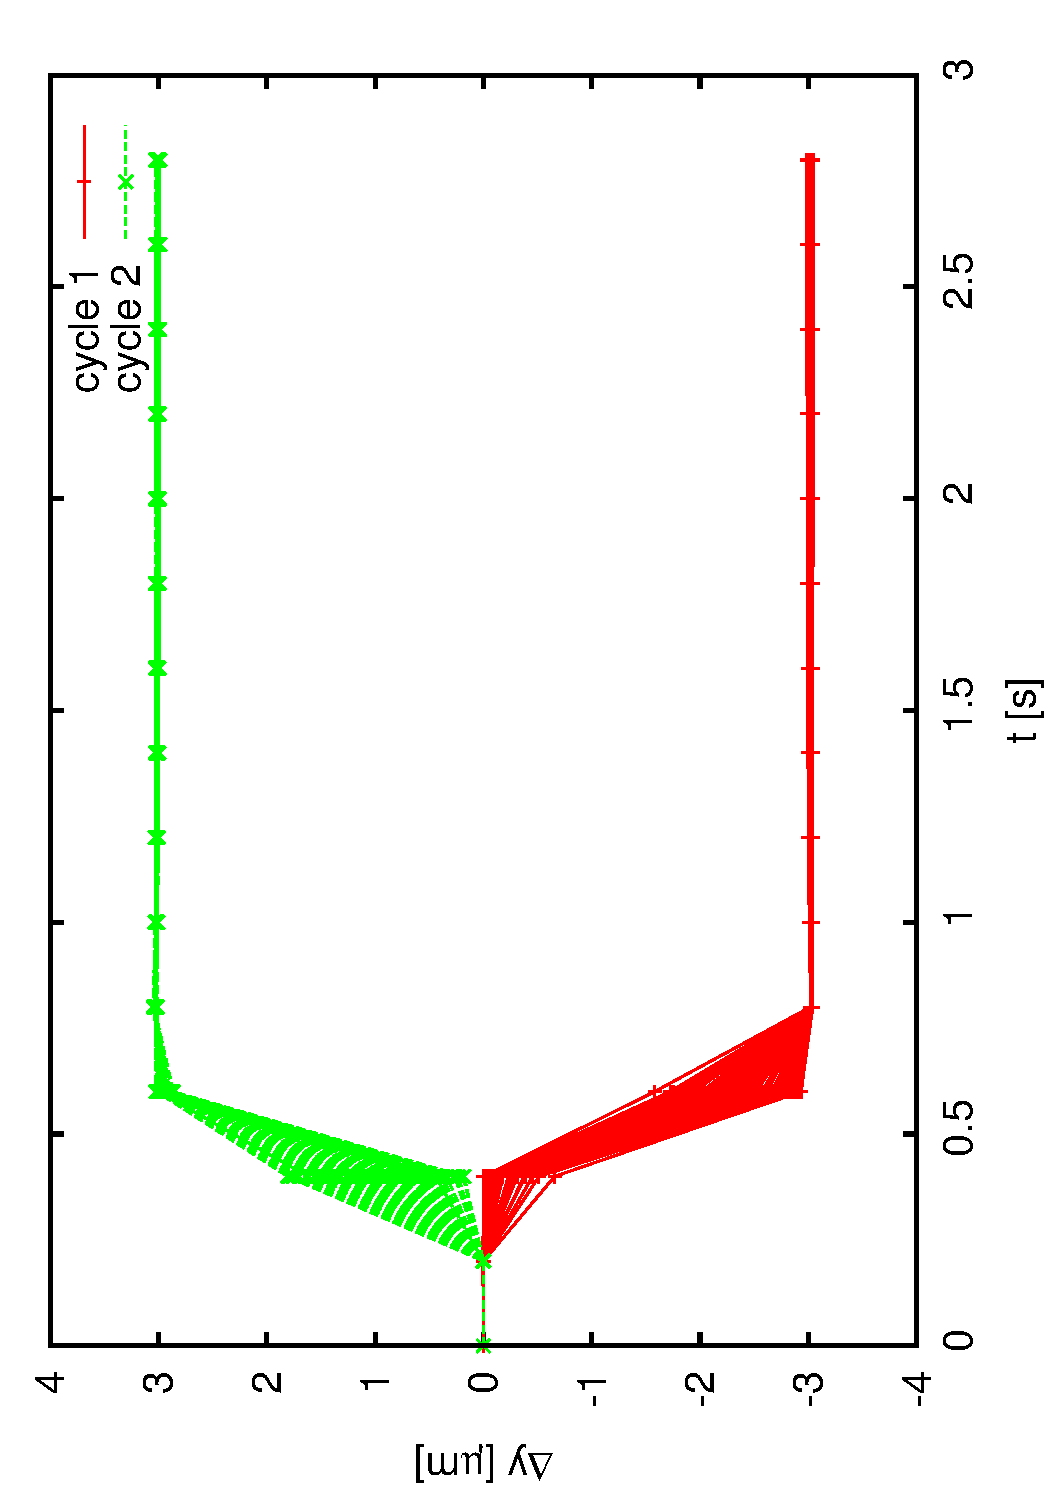
\includegraphics[angle=-90,scale=0.30]{image04.pdf}\caption{Settling speed with feedback for PI movers.}\label{f:PImsteps}
\end{subfigure}\hspace*{1.5cm}
\begin{subfigure}{0.4\textwidth}
 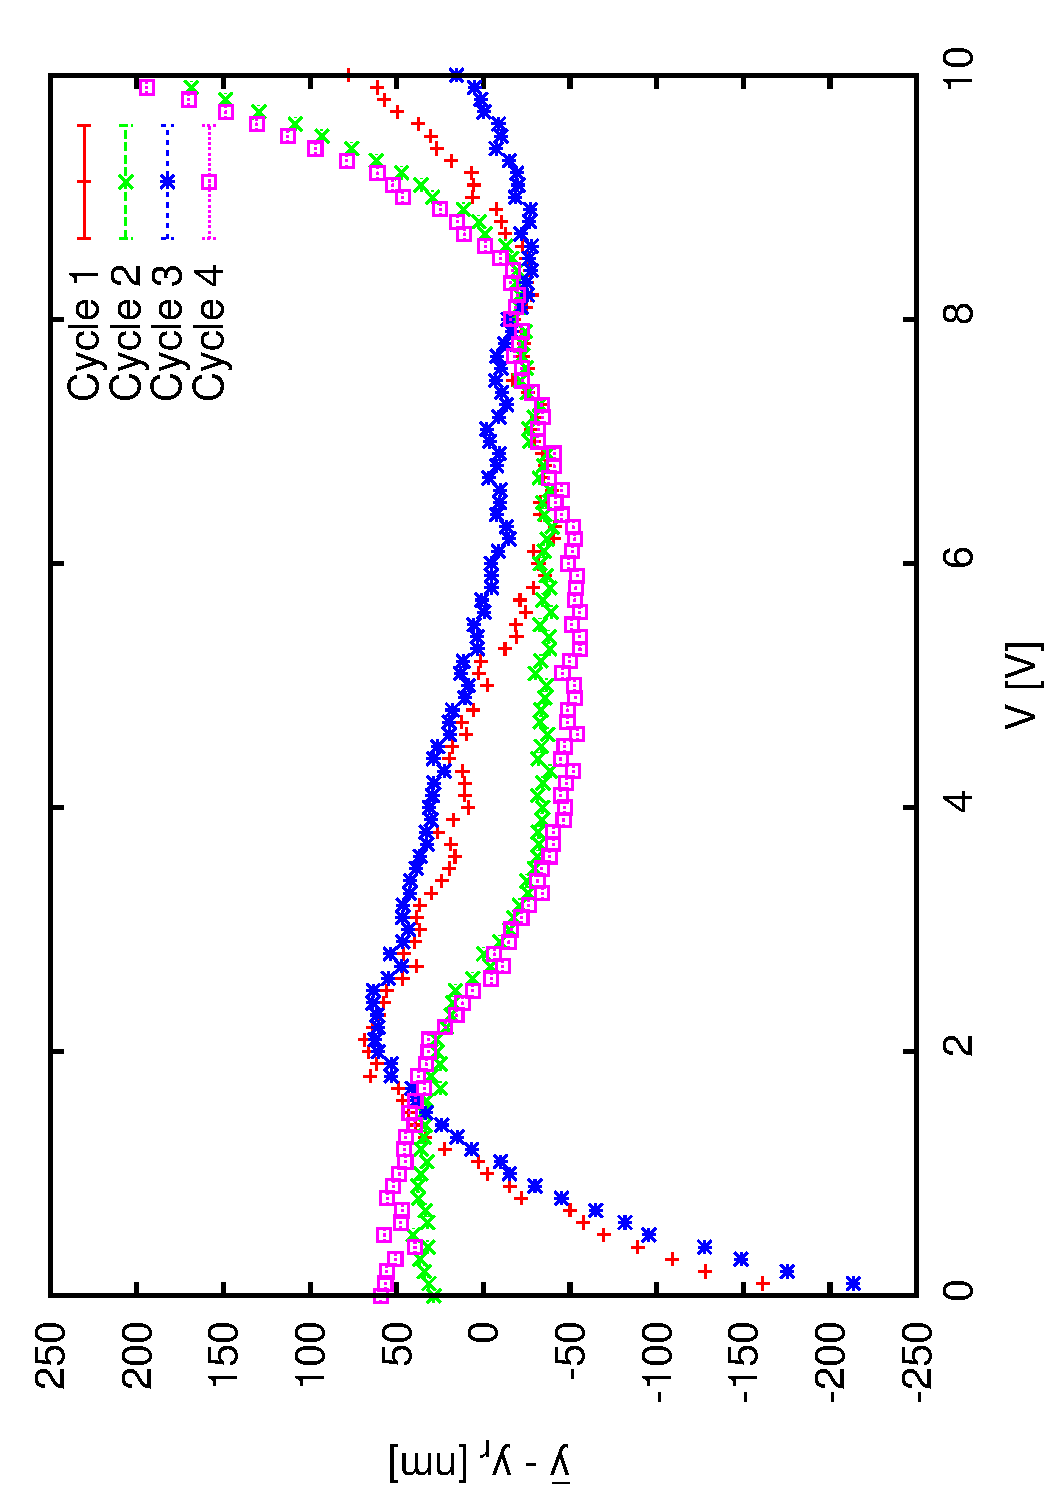
\includegraphics[angle=-90,scale=0.30]{image06e.pdf}\caption{Residual non-linearity (with fb), after substraction of linear fitting on PI movers.}\label{f:PIlinres}
\end{subfigure}\caption{Block C movers, linearity test over four cycles.}\label{f:PIfeedback}
\end{figure}
The calibration mean from these 4 cycles is $C_{mC} = (30.002\pm7)\mu$m/V. This value is valid for ranges were the residual is constant enough, therefore, it is recommended to use the movers with voltage settings in the middle of the total dynamic range and/or scan over less than 1 V.\par
The step stability was tested by moving back and forth the voltage setting hundreds of times. Fig. \ref{f:PIstepstab} shows that 20 nm steps can be resolved and Fig. \ref{f:PIstab} shows 1.13 nm of stability on each setting with feedback.\par
\begin{figure}[!htb]
 \centering\hspace*{-0.6cm}
\begin{subfigure}{0.4\textwidth}
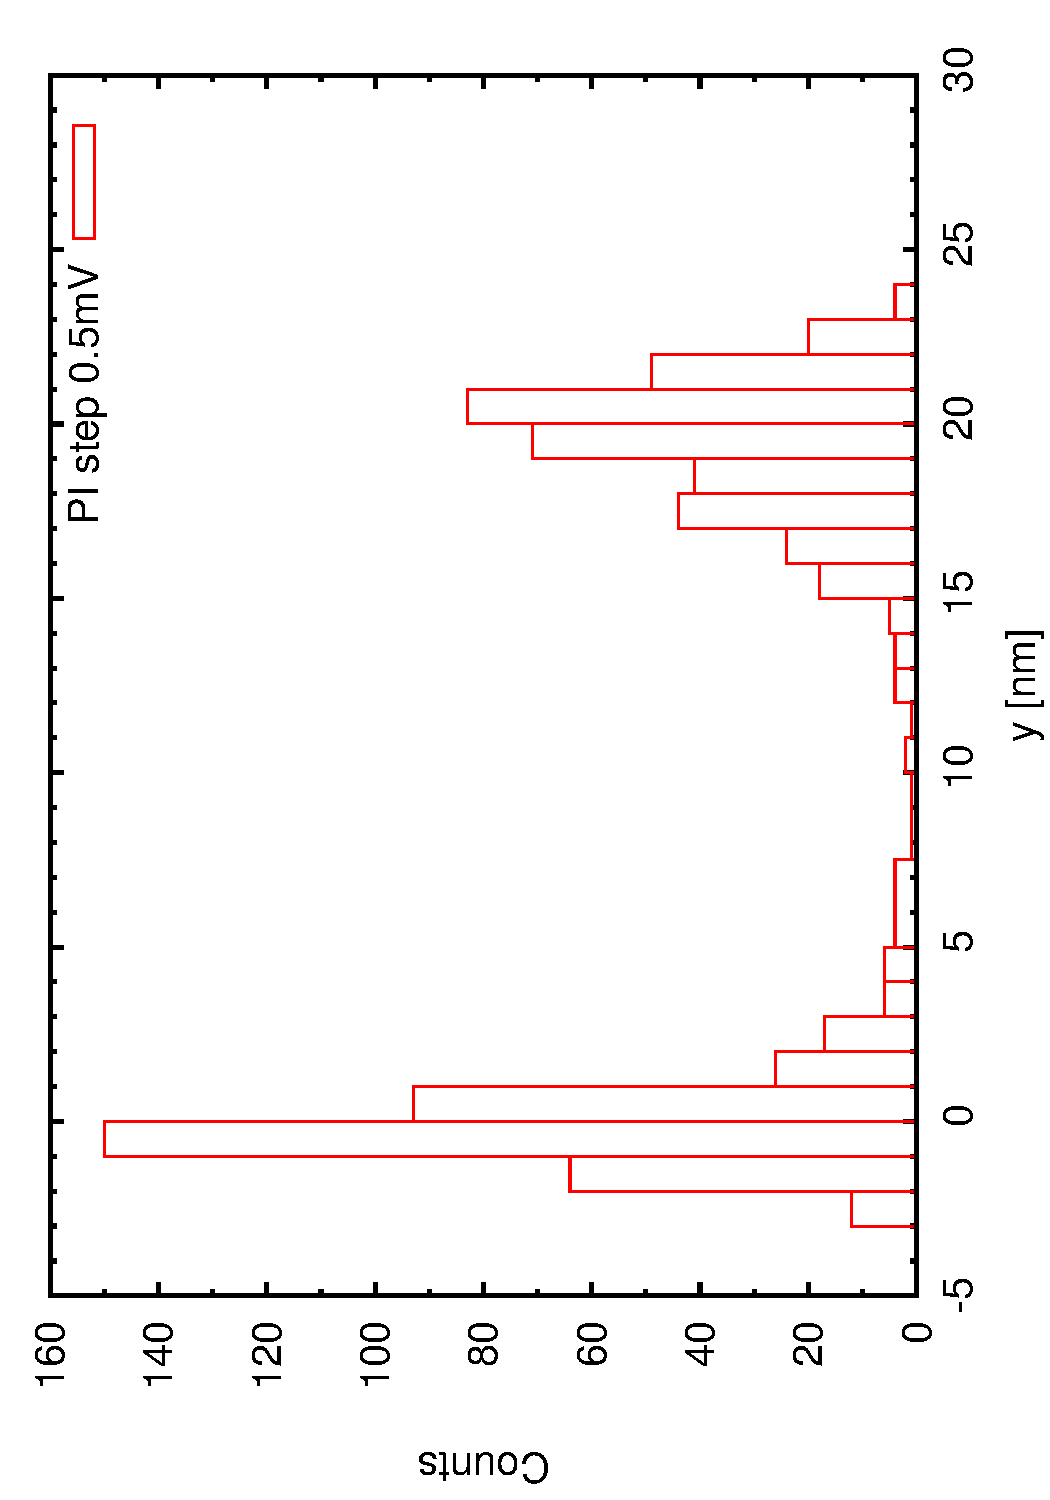
\includegraphics[angle=-90,scale=0.30]{imagestep01a.pdf}\caption{Minimum voltage setting variation back and forth tested was 0.5 mV.}\label{f:PIstepstab}
\end{subfigure}\hspace*{1.5cm}
\begin{subfigure}{0.4\textwidth}
 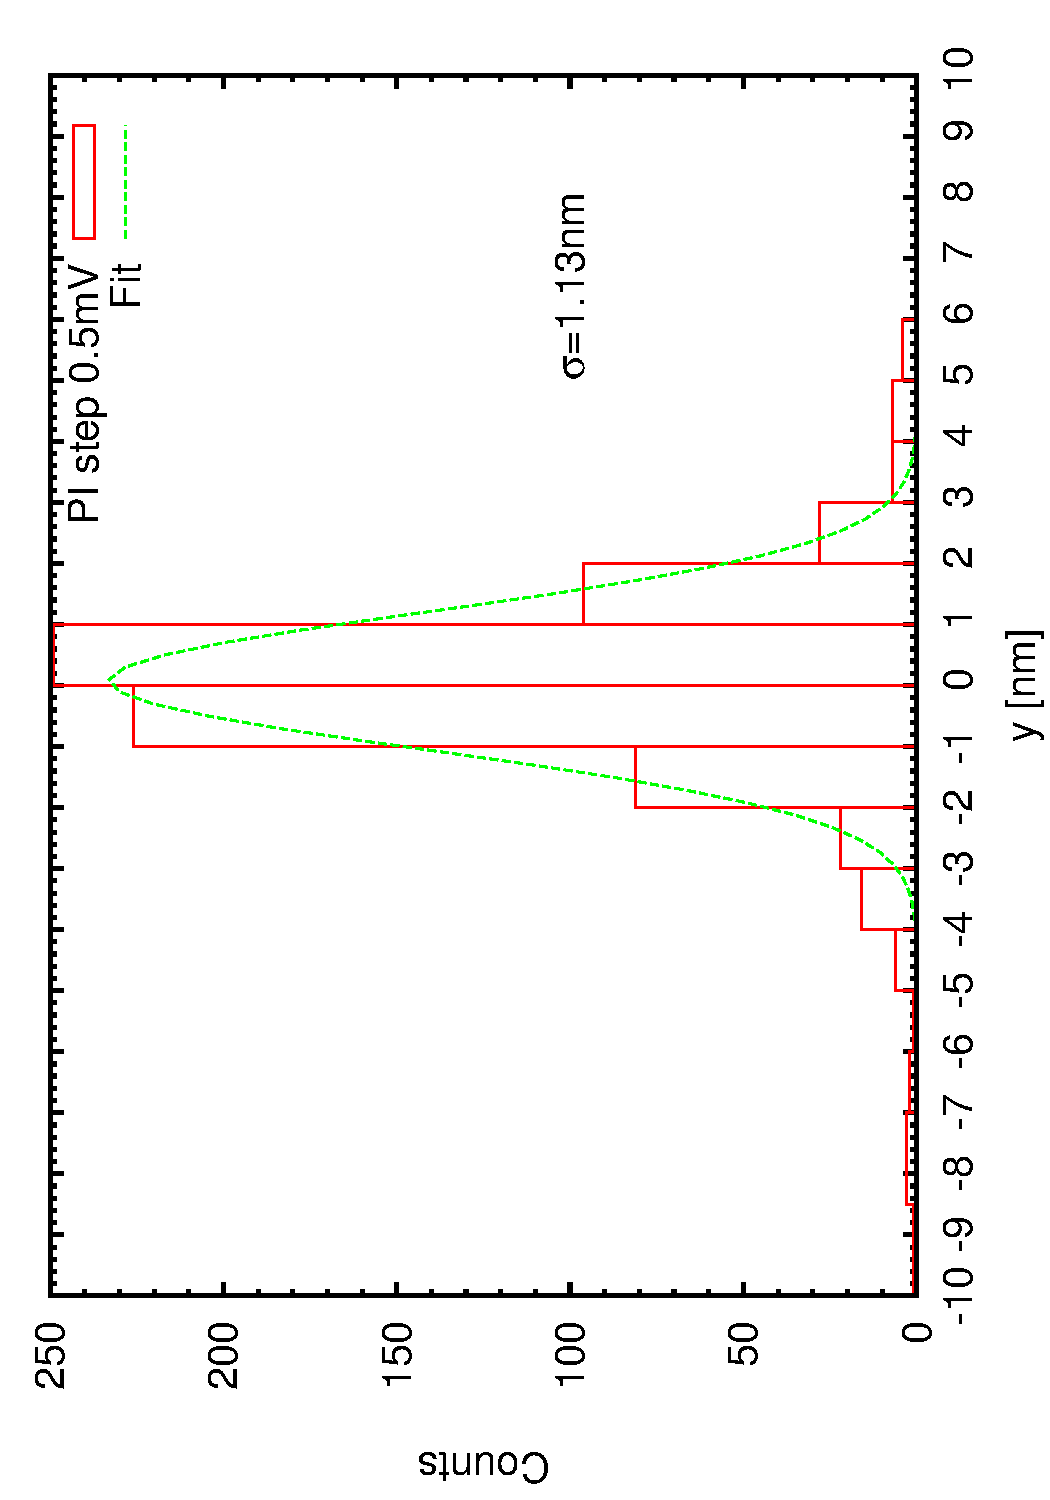
\includegraphics[angle=-90,scale=0.30]{imagestep01.pdf}\caption{Settling speed with feedback for PI movers.}\label{f:PIstab}
\end{subfigure}\caption{Stability at fixed voltage setting.}\label{f:PIstability}
\end{figure}
Coupling effect of horizontal displacement on the vertical plane was also tested. Fig (\ref{f:PIcoupling}) shows vertical position variation of 3~$\mu$m (1\%) of total horizontal dynamic range.\par
\begin{figure}[!htb]
\centering
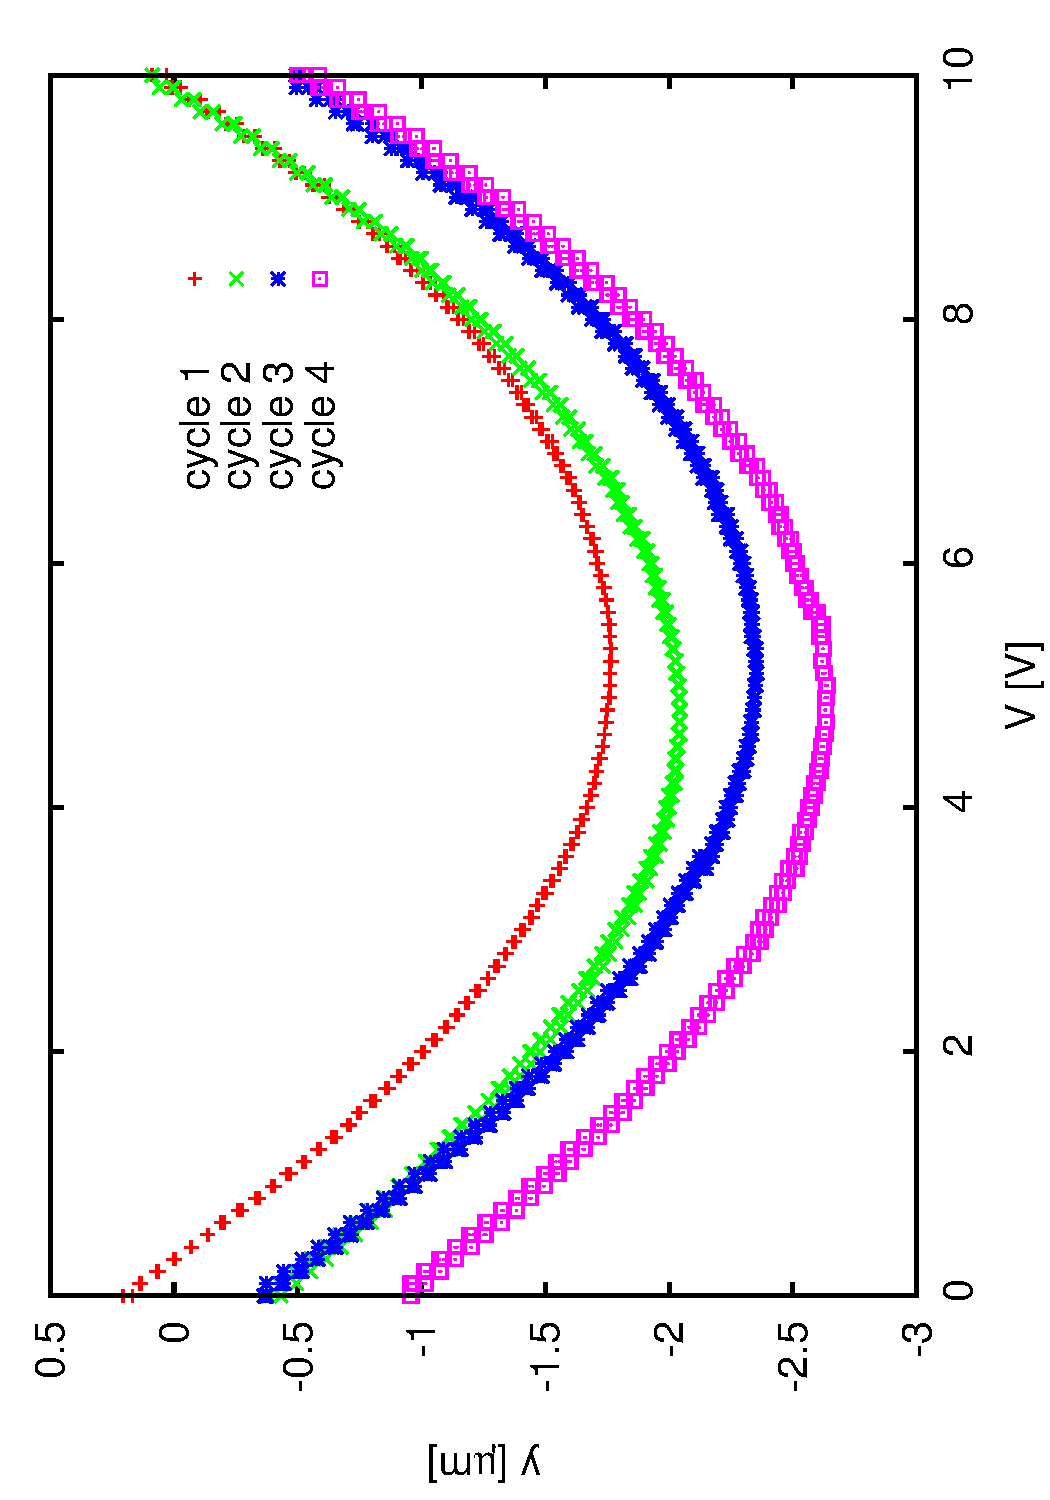
\includegraphics[scale=0.32,angle=-90]{image42.pdf}\caption{Horizontal to vertical movers coupling.}\label{f:PIcoupling}
\end{figure}
In the same way as with previous block, only the readbacks from the control box are available after installation indicating current mover position. Results from readback linearity with respect to voltage setting within ranges below 1~V show that readbacks are limited by electrical noise of $5.3$~mV limiting the calibration steps. This however does not provide information of the movers stability because the feedback loop is closed inside the control box. The noise is Gaussian, and its effect on calibration can be minimized by averaging over several readings.\par
\subsection{Cavity response calibration $C_c$}\label{s:calibration}
During beam time the cavity position is systematically changed and the amplitude of the cavity output signal is measured. Calibration is calculated from the movers voltage readbacks and choosing the signal peak from the acquired waveform,  giving the factor $C_c=I'/V$ [a.u./V], and the IQ rotation angle $\phi$.\par
Input signal can be attenuated from 0 dB to 70 dB in order to keep it inside of the electronics linear response and acquisition system limits. The system response with attenuation change can be seen in Fig. \ref{f:calatt}. The variation of the calibration is within $\pm5\%$ for charge between $(0.4\sim0.5)\times10^{10}$ particles, except for IPBy at 0~dB. The reason for this is a saturation of the electronics, as explained in Section \ref{s:dynrange}.
\begin{figure}[!htb]
 \centering\hspace*{-0.6cm}
 \begin{subfigure}{0.4\textwidth}
  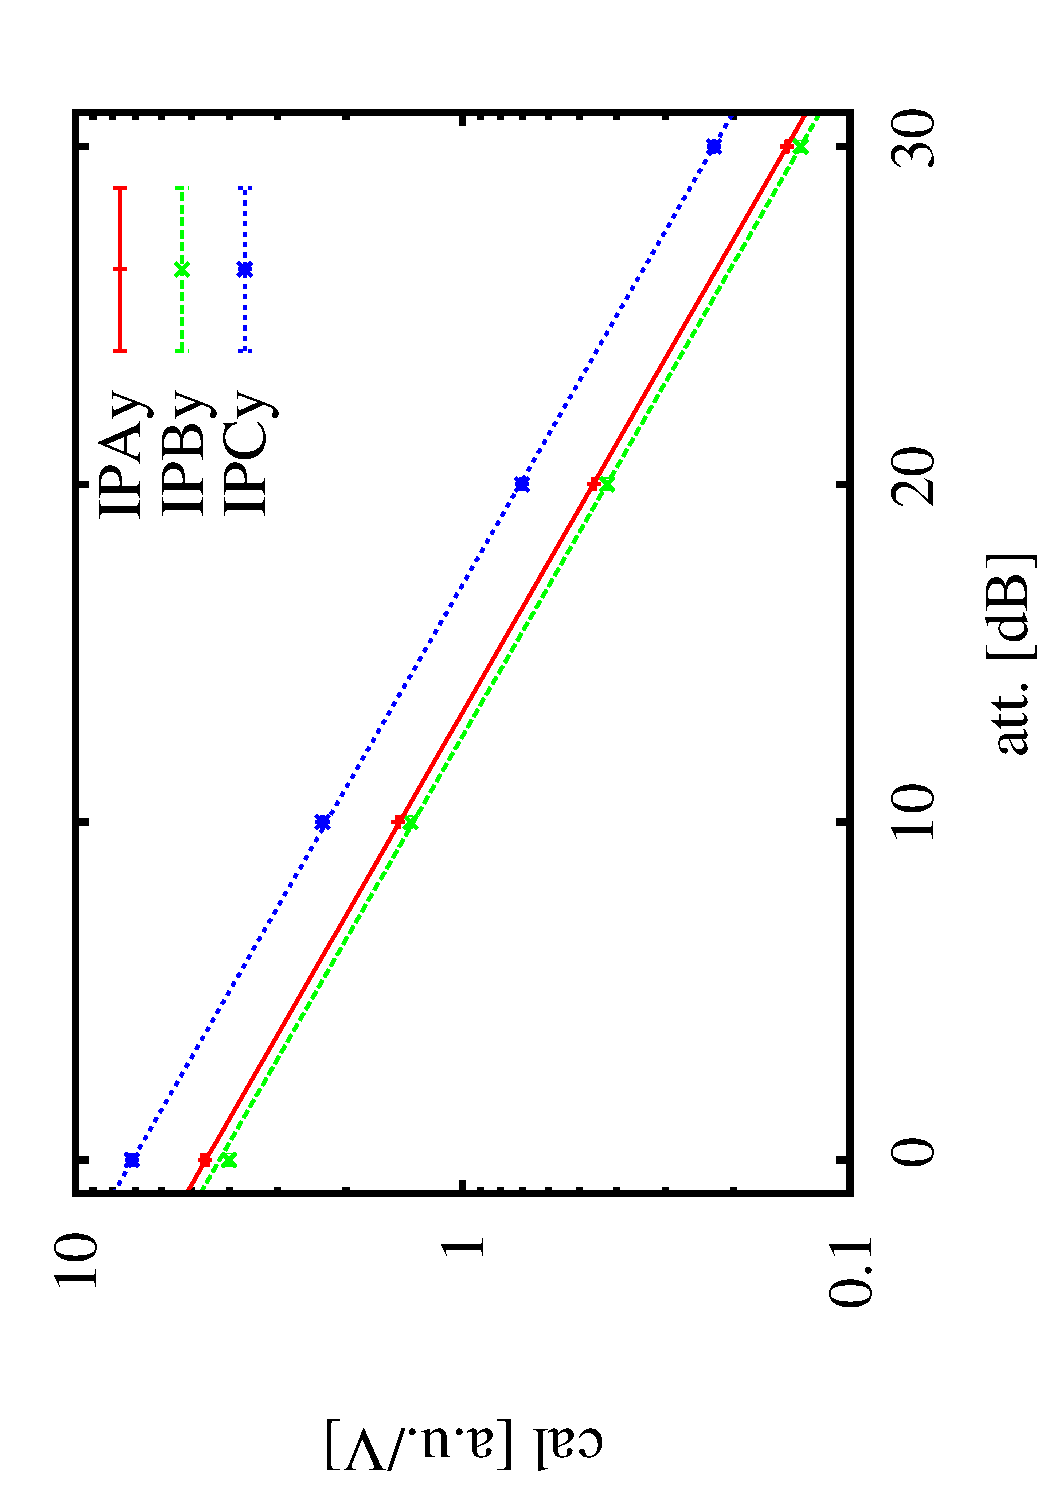
\includegraphics[scale=0.3,angle=-90]{image01_calsy.pdf}\caption{Calibrations in the vertical plane for the three BPMs.}\label{f:calsy}
 \end{subfigure}\hspace*{1cm}
\begin{subfigure}{0.4\textwidth}
  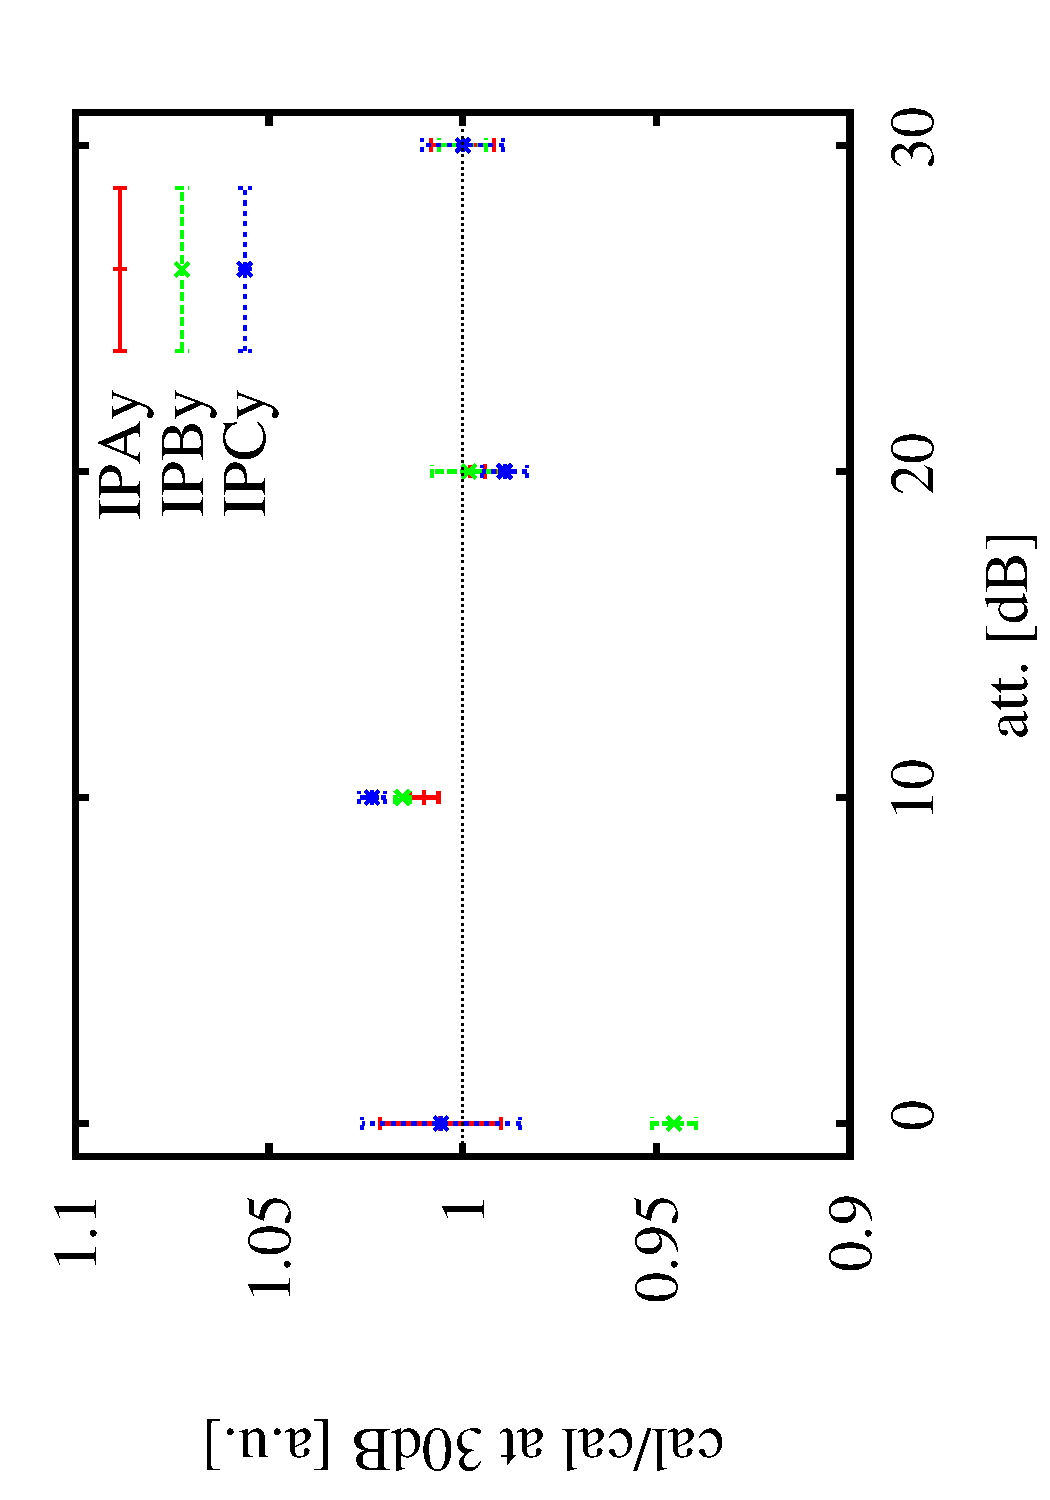
\includegraphics[scale=0.3,angle=-90]{image01_calsynorm.pdf}\caption{Vertical calibrations scaled down and normalized to the measurement at 30~dB attenuation.}\label{f:calsynorm}
 \end{subfigure}\caption{Calibrations as a function of attenuation.}\label{f:calatt}
\end{figure}

\section{Dynamic Range}\label{s:dynrange}
Dynamic range is defined in this section as the movers' voltage range in which the cavity response is linear within a tolerance, and where it therefore can be translated to position using the calibration factor, $c_m$, obtained in Sect. \ref{s:calcm}. The dynamic range is limited by the linear response of the cavity sensitivity, the processing electronics and the acquisition system.\par
\subsection{Acquisition System}
Every study case has been performed with signals inside the acquisition system dynamic range, described in \ref{s:acqsys}. The initial FONT board has been recently replaced by a dedicated SIS digitizer with larger and configurable voltage range. This is no longer a limitation.\par
\subsection{Processing electronics and cavity sensitivity}
The processing and cavity response are combined in the calibration study showing linearity within $\pm5\%$ as described in Sect.~\ref{s:calibration}. However, Fig.~\ref{f:calsynorm} shows that IPBy calibration is just outside this range at 0~dB attenuation. In order to explain this behaviour the $Q'$ signals from calibrations are shown in Fig. \ref{f:Qp}. A visible difference between IPAy and IPCy with respect to IPBy can be seen. The decay of IPAy and IPCy $Q'$ signals is consistent with system resolution studies shown in Sect. \ref{s:resolution}. However, the IPBy $Q'$ signal remains close to ($0.2\sim0.3$)~V of movers voltage in the attenuation range from 0~to~20~dB, equivalent to $(6.2\sim9.3)~\mu$m using $C_{mAB}$.\par% As the $Q'$ sensitivity derives from the $I'$ sensitivity, it shows that the IPBy signal response is constant along the three attenuation levels.\par
\begin{figure}[!htb]
\centering
 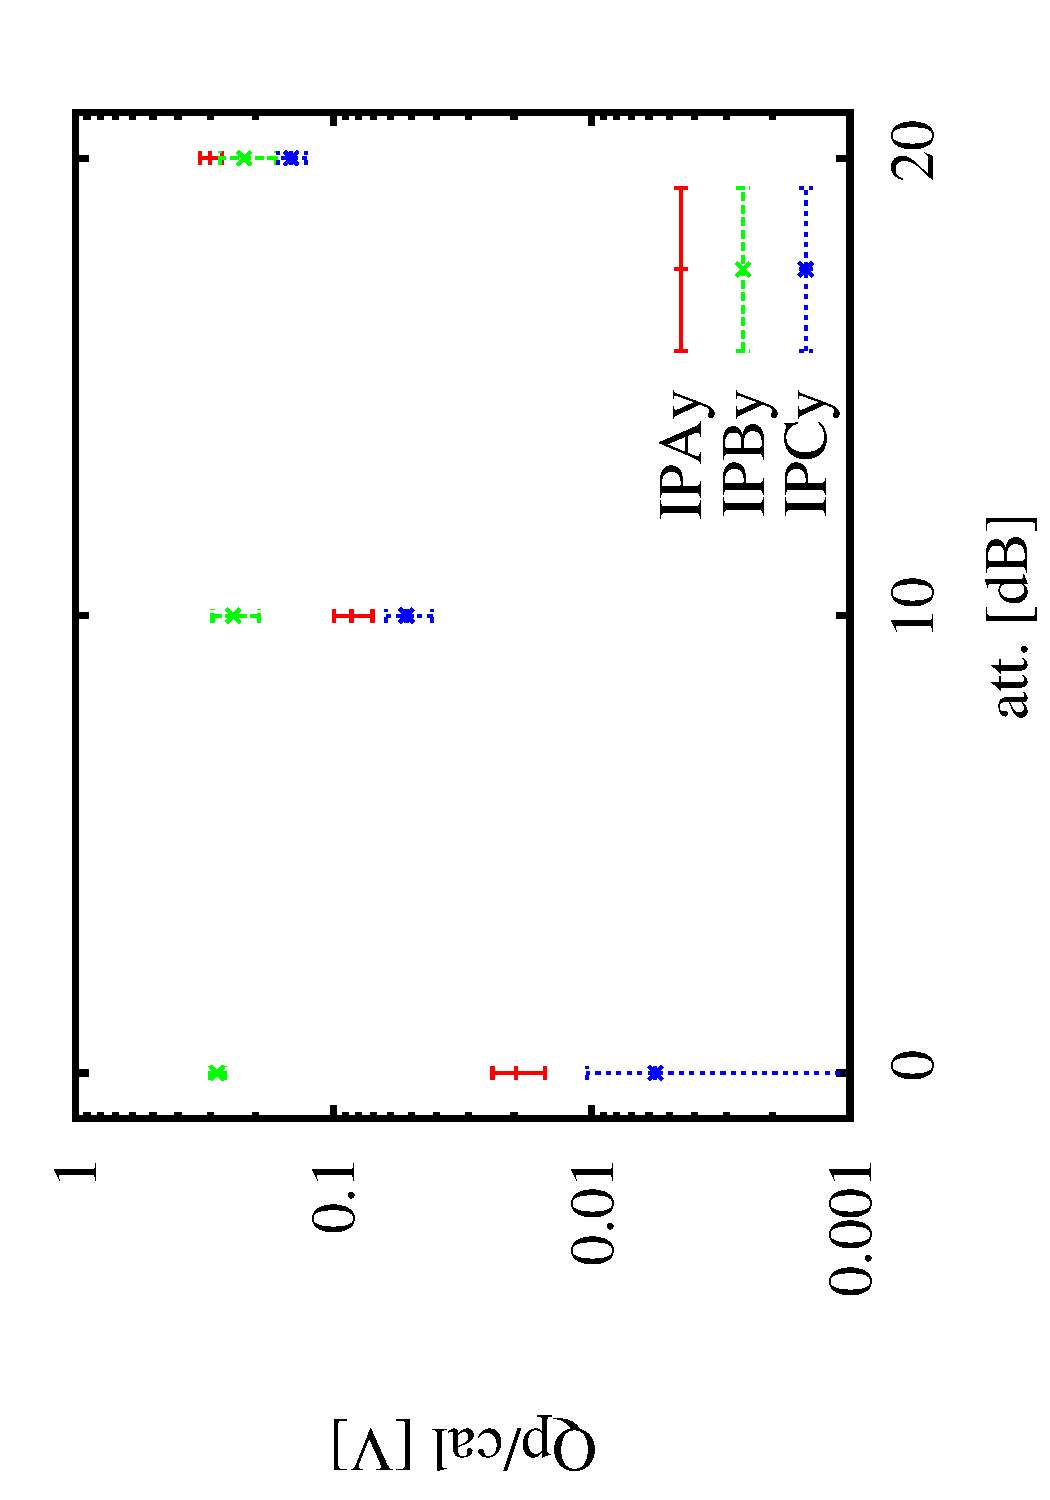
\includegraphics[scale=0.3,angle=-90]{image01_Qp.pdf}\caption{Effect of attenuation in $Q'$ signals from calibrations. Error bars are RMS.}\label{f:Qp}
\end{figure}
In the same way, the IPBy calibration versus charge is shown in Fig.~\ref{f:chargescan}, where the calibration values have been normalized to the minimum charge and attenuation is fixed at 10~dB. The calibration constant decays by more than $5\%$ at charges above $0.4\times10^{10}$ particles.\par
The maximum amplitude of the signal $A=\sqrt{I'^2+Q'^2}$ has been used to obtain the dynamic range. From the non-saturated calibration at $0.36\times10^{10}$ and 10 dB att. the signals $I'$ and $Q'$ are used to obtain $A=0.36$~V of movers range, equivalent to 11~$\mu$m using $c_{mAB}$, where the cavity calibration $c_B$ varies less than $\pm5\%$.  Similar dynamic ranges, in the order or 8~to~10~$\mu$m, have been found for IPAy and IPCy, however they lack the charge scan.\par
The IPBy~$Q'$ signal fills up almost all dynamic range at 10~dB attenuation and $0.4\times10^{10}$ particles, and it is saturating the processing electronics at 0~dB.\par
\begin{figure}[!htb]
\centering%\hspace*{-0.6cm}
% \begin{subfigure}{0.4\textwidth}
 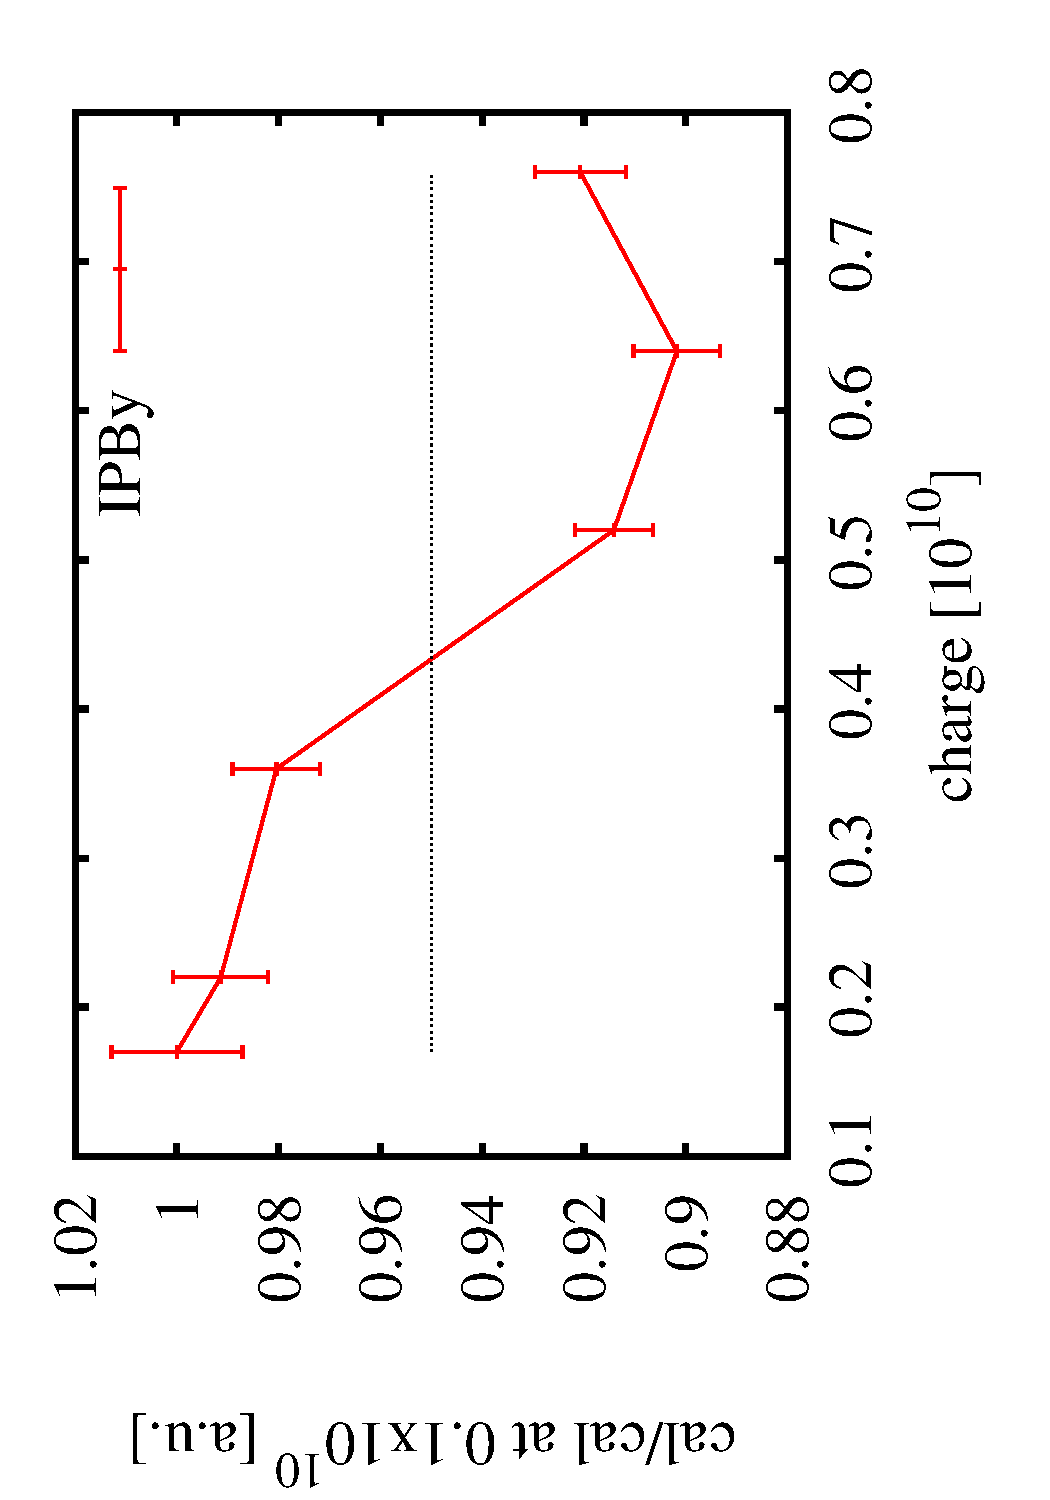
\includegraphics[scale=0.3,angle=-90]{image01_Calvscharge.pdf}\caption{IPBy Calibration versus charge normalized to the calibration at minimum charge.}\label{f:chargescan}
% \end{subfigure}\caption{Cavities $Q'$ signal and calibration charge scan for IPBy normalized to the minimum charge.}
% \hspace*{1cm}\\
% \begin{subfigure}{0.4\textwidth}
%  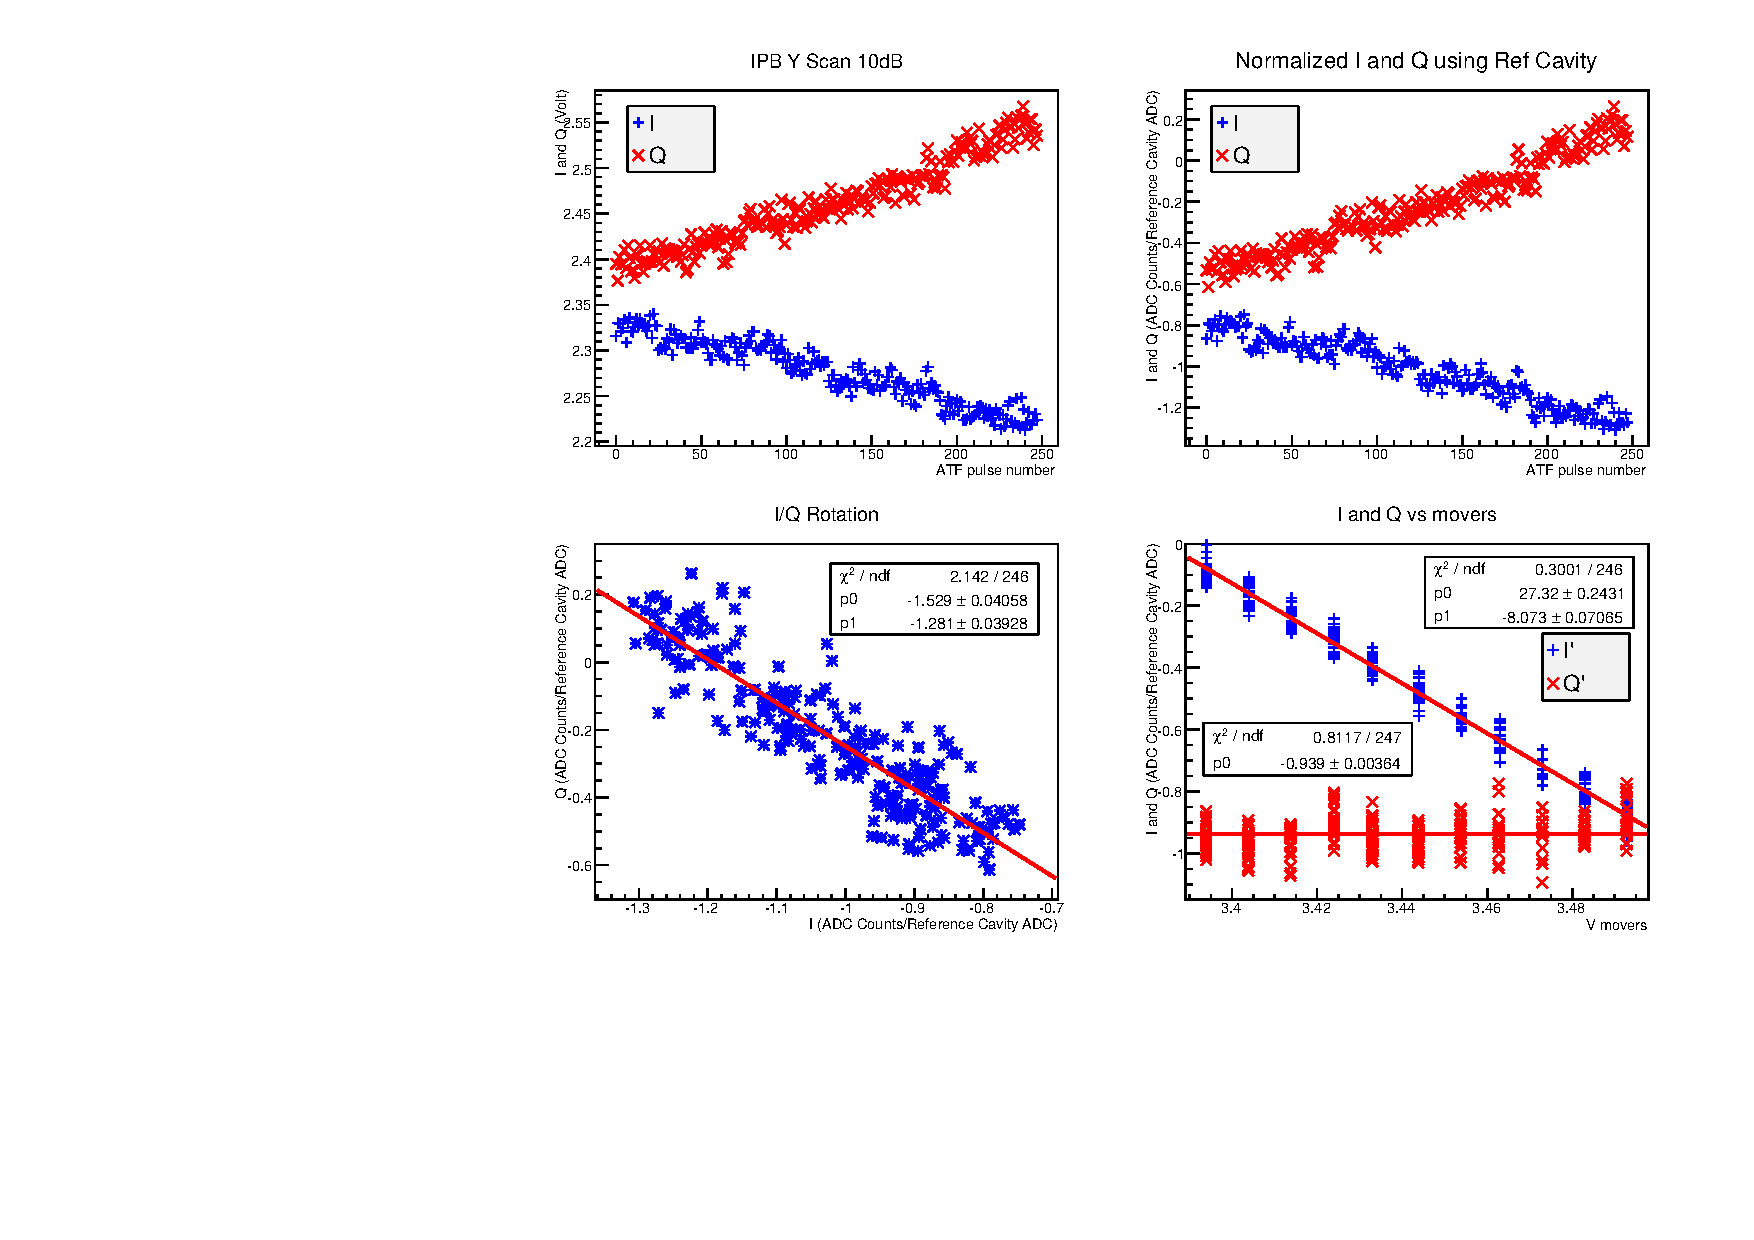
\includegraphics[scale=0.6,angle=0]{IPByCal11_10dB_sample68.pdf}\caption{Calibration at .}\label{f:IPBydynrange}
% \end{subfigure}
\end{figure}
To predict the measured dynamic range of IPBy it is necessary to put extra 6dB of attenuation in the processing electronics gain model (Sect. \ref{s:processing}) . At the moment, it has been attributed to lower than expected sensitivity of the cavities in Section \ref{s:resosensi} and/or cable loss in the processing electronics interconnection.\par

\section{Resolution}\label{s:resolution}
Resolution is measured in nm using the calibration results from Sect. \ref{s:cals}. It is limited by the cavity sensitivity, the electronics noise floor and the acquisition system resolution.\par
\subsection{Acquisition System}
The acquisition system resolution is specified in Sect. \ref{s:acqsys}. Only the oscilloscopes had lower than required resolution, however, they have already been replaced by a dedicated SIS digitizer. This is no longer a limitation.\par
\subsection{Noise floor and cavity sensitivity}
The BPMs, processing electronics and conections along the BPM signal path generate noise limiting the minimum detectable waveform. This minimum is estimated by scanning the measured jitter versus the attenuation value.\par
At large attenuations the noise floor is bigger than beam jitter at the BPM, while at low attenuations is the opposite. There is an inflection point where both are relevant. The cavity calibrations are used to translate the measurments into~nm.\par
The jitter acquisition is the measurement of bunch position over several hundreds of pulses with a fixed BPM position. 
The readings from the 3 BPMs are shown in Fig. \ref{f:resojitter}. Jitter for the three BPMs is in the order of $300\sim400$nm, consistent with true beam jitter at that day (because the beam was not tuned after a DR extraction kicker issue). At 40~dB the noise is larger than beam signal and by extrapolation the resolution limit per BPM is 13~nm for IPAy, 11~nm for IPBy, and 23~nm for IPCy at 0~dB.\par
\begin{figure}[!htb]
\centering%\hspace*{-0.6cm}
% \begin{subfigure}{0.4\textwidth}
 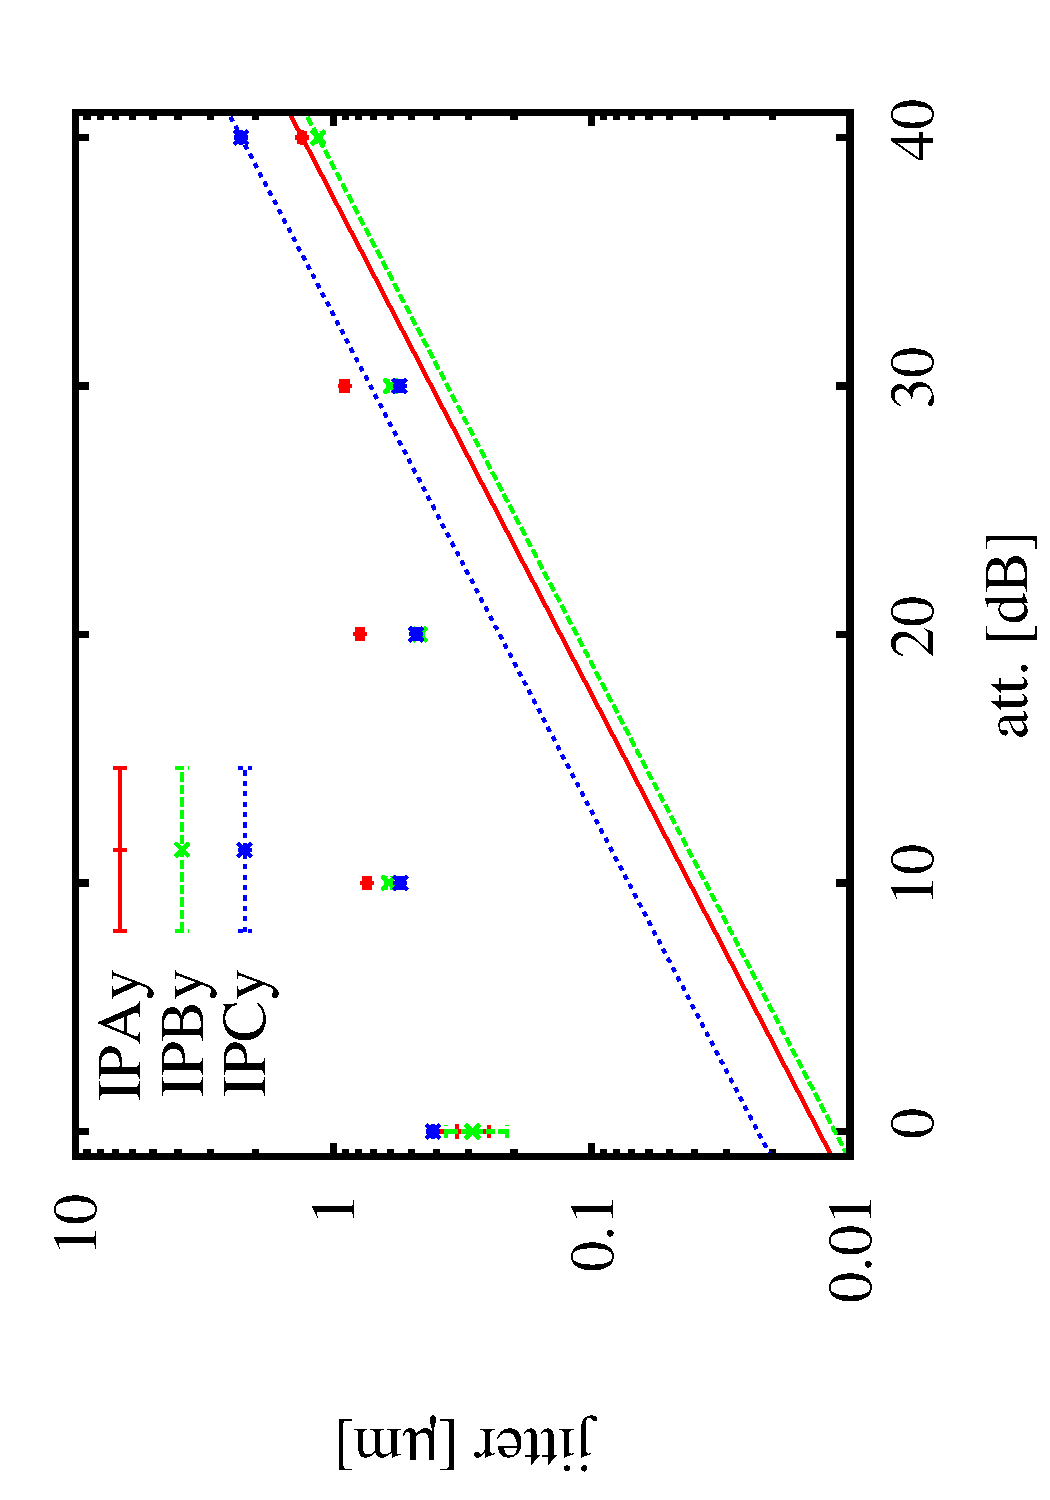
\includegraphics[scale=0.3,angle=-90]{image01_jitter.pdf}\caption{Jitter measurement for the 3 BPMs.}\label{f:resojitter}
% \end{subfigure}\hspace*{1cm}
% \begin{subfigure}{0.4\textwidth}
%  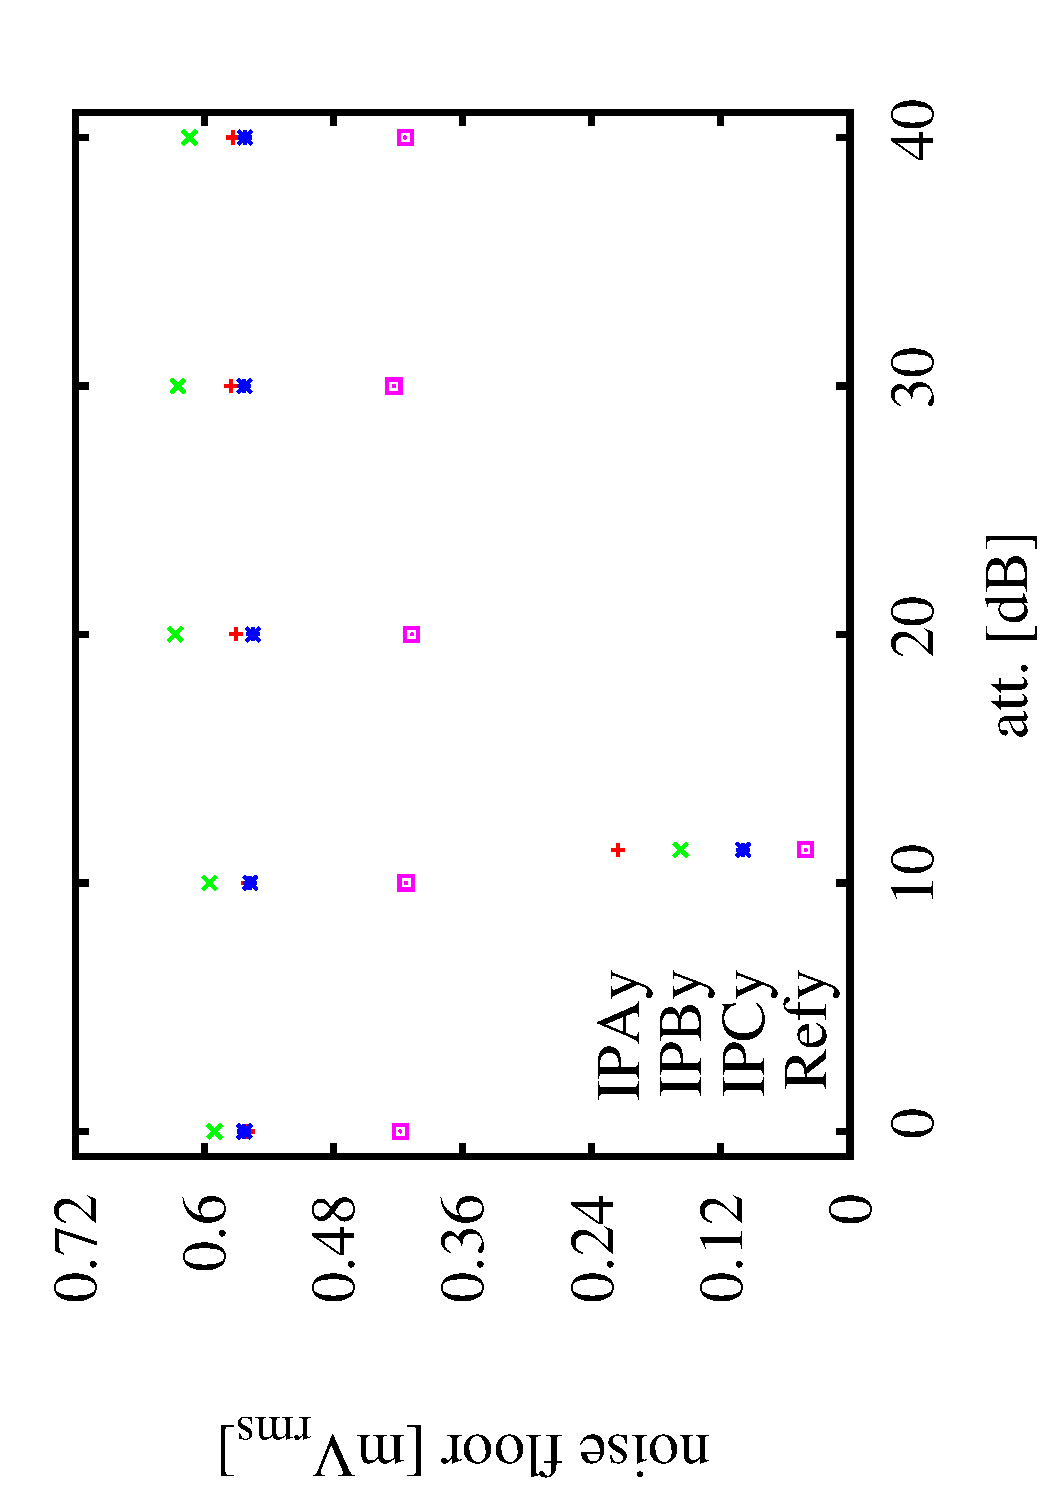
\includegraphics[scale=0.3,angle=-90]{image01_noisetot.pdf}\caption{Noise per channel for the 3 BPMs.}\label{f:resonoisetot}
% \end{subfigure}\caption{Resolution extrapolation by jitter measurement for the 3BPMs.}\label{f:resojitternoise}
\end{figure}
It is also clear that IPC shows a worse resolution limit than IPA or IPB. Two possibilities arise: the electronics noise is larger for IPC or the sensitivity is lower.\par 
\subsubsection{Noise floor}
Jitter measurements at 60~dB and 70~dB attenuation with $0.4\times10^{10}$ particles have shown that, after substraction of known gains from first, second down-mixing stages and hybrid, the noise floor value varies by only $\pm1$ dB among BPMs.\par
Although, it can not be considered a direct measurement of the processing noise floor as in \cite{PhysRevSTAB.11.062801} because additional losses are not included, it does indicate that the noise floor is similar for the three BPMs and that it is not the explanation for the discrepancy seen in Fig.~\ref{f:resojitter} between IPCy when compared to IPAy and IPBy.\par
A lower limit of 10~nm on the resolution per BPM results from the processing electronics noise floor in the current state.\par

\subsubsection{Cavity sensitivity}\label{s:resosensi}
Cavity sensitivity and processing electronics gain change the calibration factors. Due to the 6~dB mismatch between the dynamic range measured and predicted for IPBy, as shown in Sect. \ref{s:dynrange}, and the lack of charge scans for IPAy and IPCy, it is not possible to conclude about the total gain without making assumptions.\par
However, the signal decay time from waveforms gives information about the cavity performance. The measurement of the decay time $\tau$ described in Sect. \ref{s:IPBPMsignals} shows a 6~ns decay for IPCy compared to 11~ns and and 12~ns for IPAy and IPCy. This difference indicates power losses which might be attributed to partially tightened bolts during mechanical assembly of the BPM. In addition, 11~ns is short when compared with expected 17~ns from design. The effect on cavity sensitivity is still under investigation.\par
The electronics gain needs to be measured per component and losses need to be identified in order to conclude whether the noise limit comes from processing electronics or the reduced cavity power.

\subsection{Resolution by trajectory reconstruction}
The system resolution could be estimated by the reconstruction of beam trajectories. Two BPMs are used to measure the bunch position and to predict the measurement at the third BPM. The residuals difference between prediction and measurement will depend on each BPM resolution.\par
Large $\beta^*$ optics has been used to obtain similar beam jitter and dynamic range in the study of the three BPMs at the same time.\par
\subsubsection{Geometrical method}
As longitudinal distances are known within a $\pm0.1$ mm over 250~mm, i.e. better than 0.1\% precision, then, geometrical factors can be used to predict the beam trajectory \cite{Nakamura:2008}, assuming that all three BPMs have the same resolution. The advantage of this method is that it is independent from beam optics as it does not require to fit parameterss to do predictions. The following is an explanation of the method.\par
\begin{figure}[htb]
 \centering
 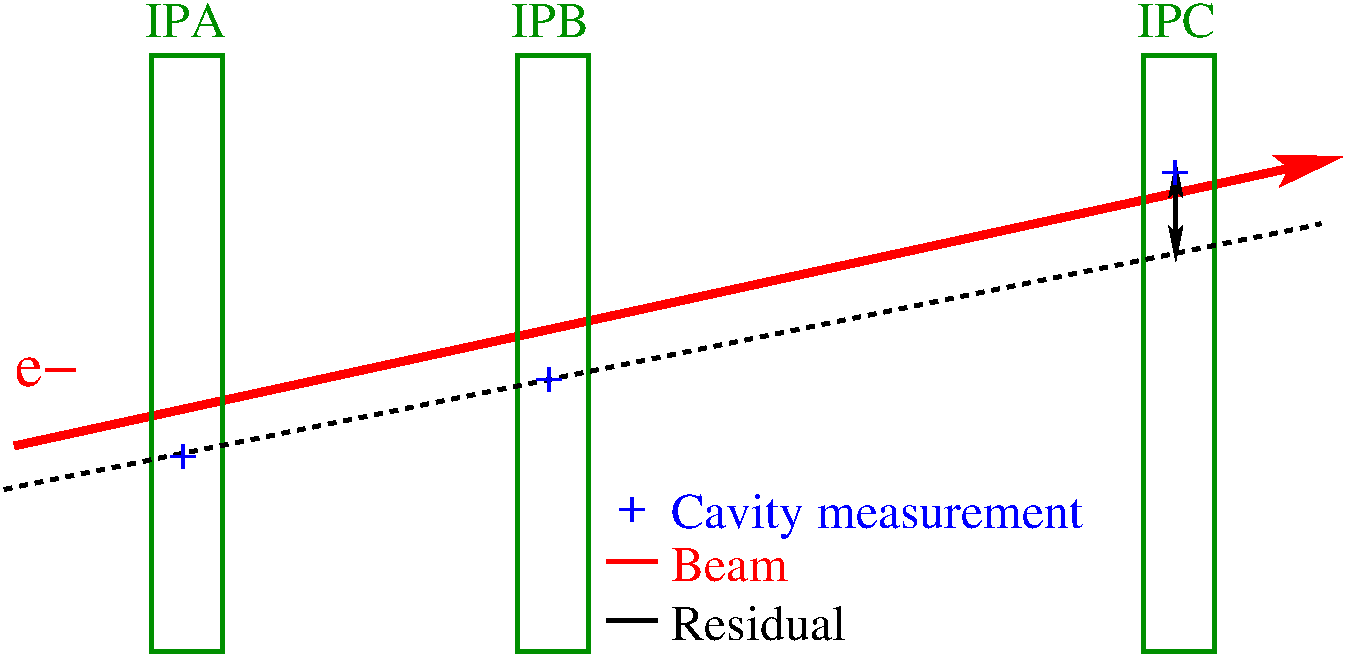
\includegraphics[scale=0.4]{resogeo.pdf}\caption{Three BPM resolution. The position measurement at IPA and IPB are used to extrapolate to IPC. The residual from substraction of the measured and extrapolated position at IPC is used to estimate the system resolution.}\label{f:3BPMreso}
\end{figure}
Being $f_C(y_A,y_B)$ the prediction at IPC from the measurement at IPA and IPB using the relative distances between the BPMs as in Fig.~\ref{f:3BPMreso}, its evaluation is substracted from the measurement in IPC as in Eq.~(\ref{eq:res}). It would be possible to calculate the theoretical propagation of uncertainty of the residual, $\sqrt{\langle R_t\rangle}$, as in Eq.~(\ref{eq:uncert}), from the individual resolution $r_A,r_B,$ and $r_c$ if they were known.\par
 \begin{align}
 R_t=& y_C - f_C(y_A,y_B)\label{eq:res}\\
  \sqrt{\langle R_t^2\rangle} =& \sqrt{\left(\frac{\partial R_t}{\partial y_A}\right)^2r_A^2+\left(\frac{\partial R_t}{\partial y_B}\right)^2r_B^2+\left(\frac{\partial R_t}{\partial y_C}\right)^2r_C^2}\label{eq:uncert}
 \end{align}
Assuming that each BPMs position measurement is independent and Gaussian distributed, the standard deviation of the residuals distribution $\sigma_{Rm}$ from measurements should be equal to the theoretical value $\sqrt{\langle R_t^2\rangle}$. Equation (\ref{eq:allr}) becomes Eq. (\ref{eq:samer}) by assuming that each BPM has the same resolution $r_A=r_B=r_C=r$. The factor in the square root in Eq. (\ref{eq:samer}) does no longer contain any unknowns, as $R_t$ is a linear extrapolation using distances, and it will be a constant, $g$, multiplying the standard deviation from measurements to estimate the BPM resolution $r$. This constant is known as the \emph{geometrical factor}.\par
\begin{align}
 \frac{\sigma_{Rm}}{\sqrt{\langle R_t^2\rangle}}&=1\\
 \frac{\sigma_{Rm}}{\sqrt{\left(\frac{\partial R_t}{\partial y_A}\right)^2r_A^2+\left(\frac{\partial R_t}{\partial y_B}\right)^2r_B^2+\left(\frac{\partial R_t}{\partial y_C}\right)^2r_C^2}}&=1\label{eq:allr}\\
 \frac{\sigma_{Rm}}{\sqrt{\left(\frac{\partial R_t}{\partial y_A}\right)^2+\left(\frac{\partial R_t}{\partial y_B}\right)^2+\left(\frac{\partial R_t}{\partial y_C}\right)^2}}&=r\label{eq:samer}\\
 g\sigma_{Rm}&=r
\end{align}
The equations used for position prediction are shown in Eq.~(\ref{eq:pred}), where the coeficients are calculated from the longitudinal distance among BPMs.\par
\begin{align}
 f_A(y_B,y_C)=&1.463y_B -0.463y_C\notag\\
 f_B(y_A,y_C)=&0.683y_A +0.317y_C\notag\\
 f_C(y_A,y_B)=&-2.156y_A +3.156y_B\label{eq:pred}
\end{align}
Following the same example with IPC, it is possible to plot the measured value versus the prediction to find the slope and correlation. Ideally, both, slope and correlation are one, however they are resolution limited.\par
Being $C_m$ the measured value at IPC, $C_p$ the predicted value at IPC from the measurement in other cavities, and $R=C_m-C_p$ the residual from substraction, it is possible to obtain the slope, $m$, as in Eq. (\ref{eq:slope}). The factor $\langle  C_m\cdot R\rangle$ indicates the over or under prediction of the measurement at IPC.
\begin{equation}
 m=1-\frac{\langle C_m\cdot R\rangle}{\langle C_m^2\rangle}\label{eq:slope}
\end{equation}
% The correlation can be approximated as in Eq. (\ref{eq:corr}). If the factor $\langle  C_m\cdot R\rangle$ is small, then, the ratio $\langle R^2\rangle/\langle C_m^2\rangle$ shows how big is the residual with respect to the beam jitter.\par
% \begin{equation}
%  cor^2(Cm,Cp)\approx 1-\left(\frac{\langle R^2\rangle}{\langle C_m^2\rangle}-\frac{\langle C_m\cdot R\rangle^2}{\langle C_m^2\rangle^2}\right)\label{eq:corr}
% \end{equation}

\begin{figure}[!htb]
\centering%\hspace*{-0.6cm}
% \begin{subfigure}{0.4\textwidth}
 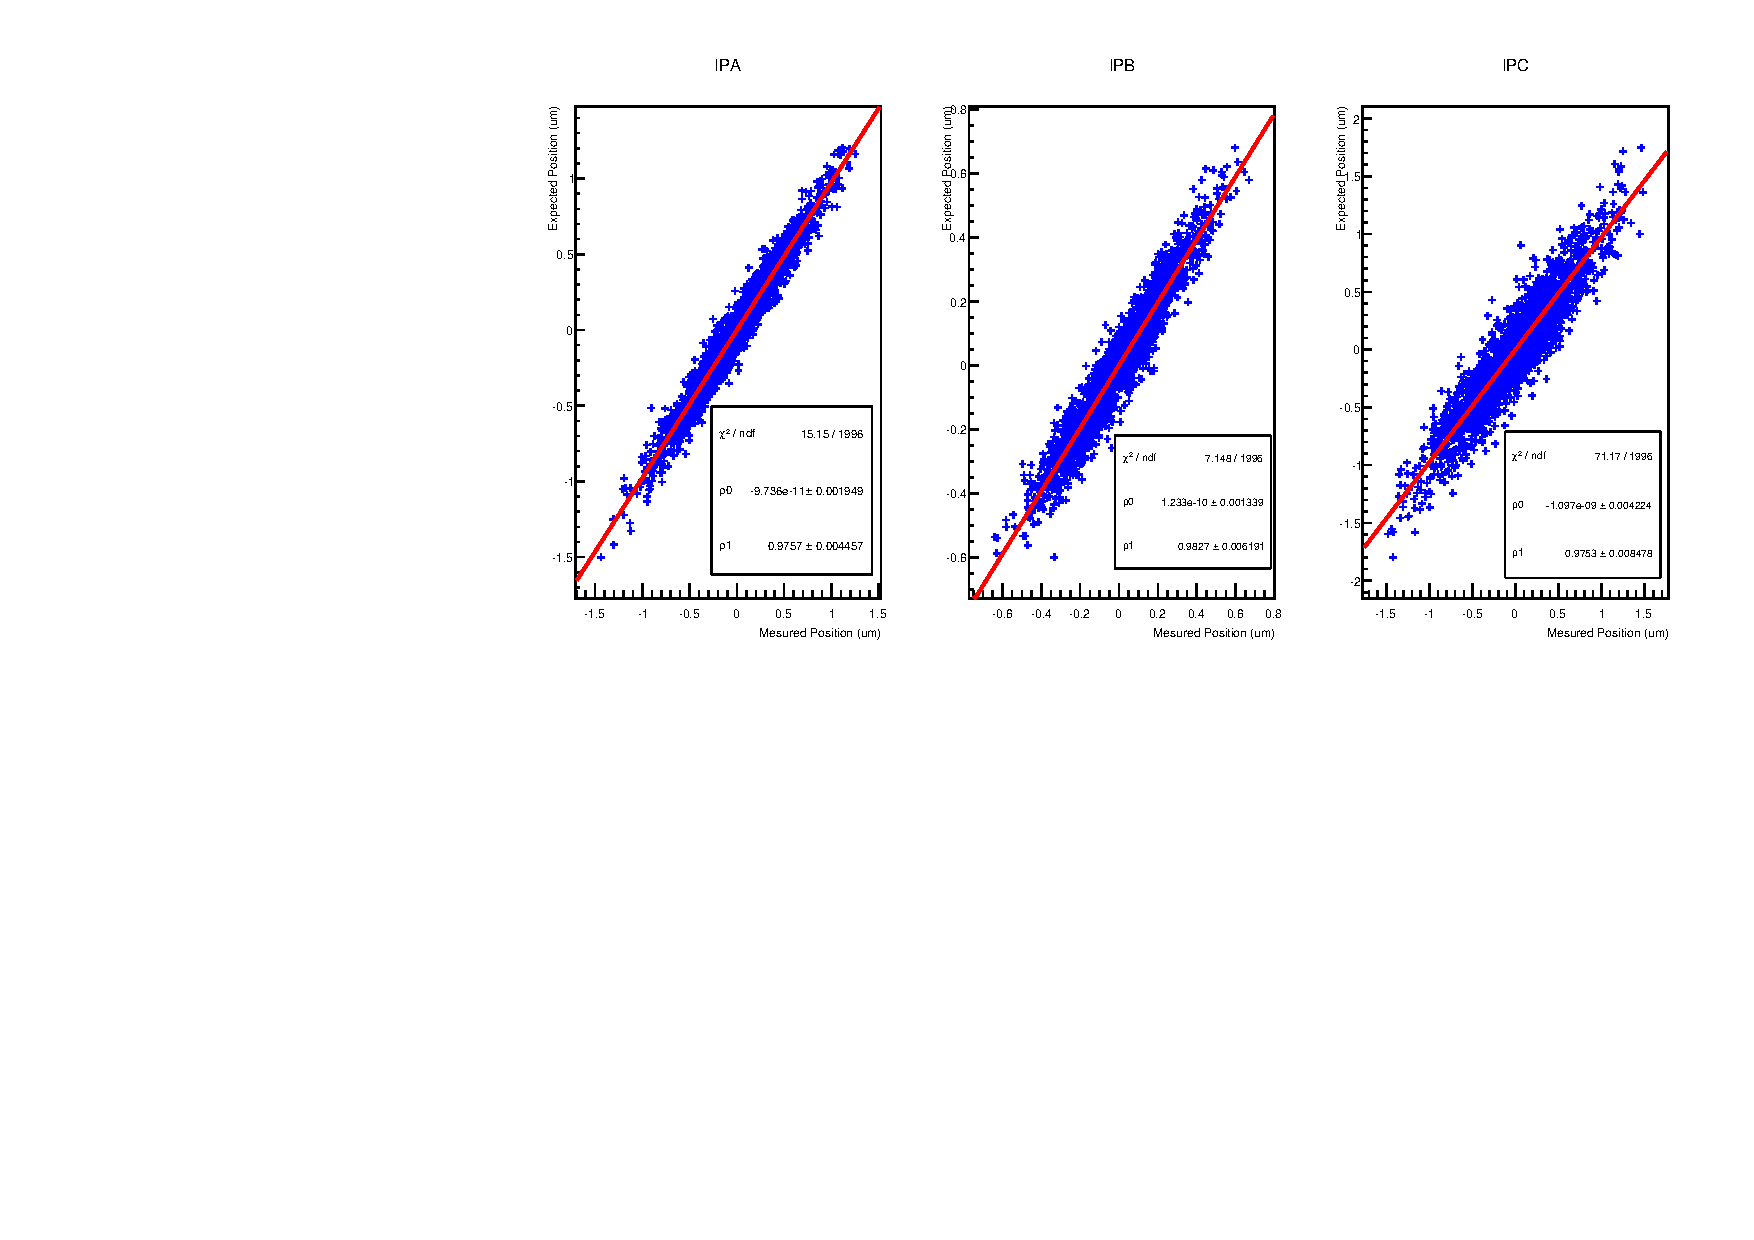
\includegraphics[scale=0.8,angle=0]{3BPM_Measured_Predicted_changing_cals.pdf}\caption{Correlation of the three BPMs measurements and predictions.}\label{f:3BPMpredictions}.
% \end{subfigure}\hspace*{1cm}
% \begin{subfigure}{0.4\textwidth}
%  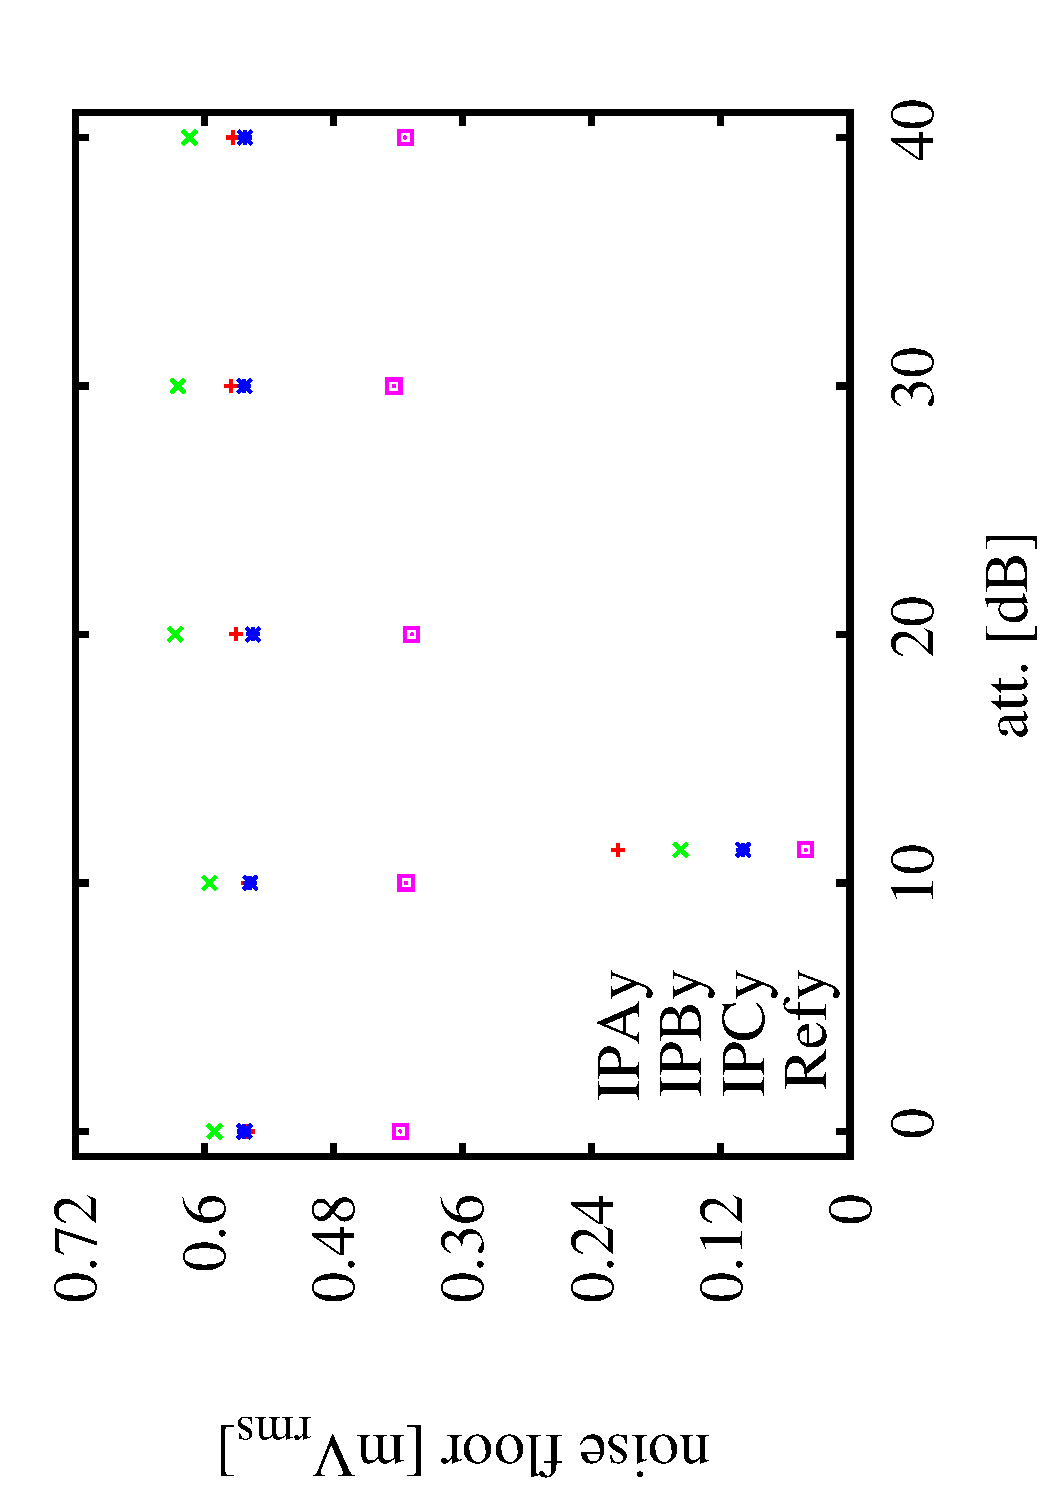
\includegraphics[scale=0.3,angle=-90]{image01_noisetot.pdf}\caption{Noise per channel for the 3 BPMs.}\label{f:resonoisetot}
% \end{subfigure}\caption{Resolution extrapolation by jitter measurement for the 3BPMs.}\label{f:resojitternoise}
\end{figure}
Figure \ref{f:3BPMpredictions} shows the correlation between the measured and predicted position at $4\times10^{10}$ particles per bunch and 0~dB attenuation, where calibration has been modified by +3.7\%, +10.9\% and -2.8\% for IPAy, IPBy and IPCy respectively in order to obtain unitary slopes within 2\%.\par
The large correction made in the IPBy calibration could be explained by the results shown in Sect. \ref{s:calibration}, and the others lay within calibration precision limits.\par
The measured jitter and the residuals from substracting the predicted value are gaussian. The jitter values, slopes and correlations of predicted vs measured positions, and geometrical factors are shown in Table \ref{t:resodata}.\par
The resolution per BPM estimated with this method by calculating the residuals on each one of the three BPMs is $(47.4\pm0.8)$ nm.\par
\begin{table}[hbt]
\centering
\begin{tabular}{c||c|c|c}\hline
Parameter & IPAy & IPBy & IPCy\\ \hline\hline
Jitter [$\mu$m] & 0.437 & 0.216 & 0.498\\\hline
Slope & $0.9757\pm0.0044$ & $0.9827\pm0.0062$ & $0.9753\pm0.0085$\\\hline
Correlation & 0.9798 & 0.9626 & 0.9322 \\\hline
Geometrical factor & 0.5457 & 0.7988 & 0.2531\\\hline
R [nm] & $87.2\pm1.4$&$59.7\pm1.0$ & $185.3\pm2.9$\\\hline
Resolution [nm] & $47.6\pm0.8$ & $47.7\pm0.8$ & $46.9\pm0.7$ \\\hline
\end{tabular}\caption{Results from trajectory reconstruction.}\label{t:resodata}
\end{table}
% \subsubsection{Optics Phase Advance}
% The optics phase advance $\phi$ is estimated by measuring the position jitter correlations among BPMs and Table \ref{t:phaseadv} shows the result of jitter correlation and phase advance between pairs of BPMs.\par
% \begin{table}[htb]
% \centering
% \begin{tabular}{c||c|c|c}\hline
% Parameter & IPAy to IPBy & IPBy to IPCy & IPAy to IPCy\\ \hline\hline
% Jitter correlation & 0.84 & -0.24 & -0.69\\\hline
% Optics Phase Advance & 33\textdegree & 103\textdegree & 134\textdegree\\\hline
% \end{tabular}\caption{Jitter correlation and estimated phase advance for the 3 BPMs.}\label{t:phaseadv}
% \end{table}
% Jitter can be decomposed in cos-like and sin-like jitter, therefore BPM resolution affects separately the trajectory reconstruction of each component due to phase advance. Being $r_{i}$ the measurement resolution at one BPM, and $r_{j}$ and $r_{k}$ the resolutions of BPMs $j,k$ used for extrapolation, the system resolution $r_s$ can be estimated from the individual resolutions by addind in quadrature the reconstruction errors from the cos-like and sine-like components, as in Eq. (\ref{eq:resos}).\par
% \begin{equation}
%  r_s=\sqrt{(r_{i}+r_{j}|\cos\phi_{ij}|+r_{k}|\cos\phi_{ik}|)^2+(r_{i}+r_{j}|\sin\phi_{ij}|+r_{k}|\sin\phi_{ik}|)^2}\label{eq:resos}
% \end{equation}
% Using the resolution limits estimated from noise limit for the 3 BPMs, Eq. (\ref{eq:resos}) is used to calculate the system resolution at each BPM. Results are shown in Table \ref{t:resos}.
% \begin{table}[htb]
% \centering
% \begin{tabular}{c||c|c|c}\hline
% Parameter & IPAy & IPBy & IPCy\\ \hline\hline
% Resolution $r_i$ [nm] & 13 & 11 & 23\\\hline
% Resolution $r_s$ [nm] & 52 & 49 & 55\\\hline
% \end{tabular}\caption{Estimated resolution limit per BPM and system.}\label{t:resos}
% \end{table}
% The IPBy system resoltion result is the closest to the geometrical result, this is justified because it has the best individual resolution and the phase advances allow to predict cos-likes almost only from IPAy and sin-likes almost only from IPCy.\par
% It is worth noting that the optics here used is an special case where the focus is diluted. With the nominal optics the phase advance between BPMs is close multiples of $\pi$ making the individual resolution to add up linearly and therefore, the system resolution would be 47 nm, matching the geometrical result.
\section{Feedback}
During recent tests, a two bunch beam train was used with a bunch spacing of 215.6 ns, and the signals from IPBy were input to the feedback system. Feedback has been tested by the FONT Group \cite{FONTfb:2015} obtaining a reduction of beam jitter down to 67 nm, compatible with the resolution shown in Section \ref{s:resolution}.
\section{Present Status and Prospects}
Table (\ref{t:IPBPMsStatus}) show a summary of the current IP-BPM results.\par
\begin{table}[hbt]
\centering
\scriptsize
\begin{tabular}{l|l|l|p{6cm}}\hline
PARAMETER & REQUIREMENT & STATUS & Comments\\\hline\hline
Resolution & $\sim$nm@$1\times10^{10}$ & <50nm@$0.4\sim0.5\times10^{10}$ & Calibration factors within 5\% linearity\newline BPM/Electronics noise : 10~nm per cavity\newline IPC sensitivity and/or gain : +20nm \newline X to Y coupling is still unexplored\\\hline
Dynamic Range & $\sim$10$\mu$m+extra@0~dB~att.& $9\sim11\mu$m@10~dB att. & Cavity response is linear within 5\%\newline Electronics starts to saturate\newline at $0.4\times10^{10}$@10~dB att.\newline IPBy Q' signal saturates at 0~dB\\\hline
Compatibility & IPBSM, EPICS & In progress &Calibration Software : Initial version released and in use. Requires comparison with offline results.\newline Jitter analysis Software : Initial version released and in use. Requires comparison with offline analysis.\newline IP-BSM, requires study of resolution vs low charge, $0.1\sim0.5\times10^{10}$ \\\hline
Feedback & Operative & Tested	& Jitter reduction to 67 nm.\newline Limited by BPM resolution.\\\hline
\end{tabular}\caption{IPBPMs status.}\label{t:IPBPMsStatus}
\end{table}
The efforts to improve over the results listed above are continuous. Precisely now, two improvements have been done on the system. First, the horizontal and vertical planes can be analyzed simultaneouly, such that data can be checked for coupling from one plane to another. Second, filters are added to the system in order to reduce the effect of the mismatch between frequencies in the down-mixing process.\par
At the moment, the first limitation to improve the resolution is the noise limit. The target is to explore the origin of the noise and characterize the gain along the signal path. That will allow to conclude on the cavity sensitivity.\par
The IPBy Q' signal is a second limitation to avoid saturation and inaccurate calibration. The reason is unknown for the moment, but it could be generated by an angular misalignment between cavities or a large static monopole signal. I think the monopole would affect also the horizontal plane too, therefore the upgraded electronics will help to diagnose this aspect.\par
In all cases, the electronics needs to be upgraded because it saturates at half the bunch charge required. Extra dynamic range in electronics for residual Q' signals would solve the problem.\par
Under current conditions the characterization of the resolution at low charges is possible, if data are synchronized with the IP-BSM system, then it will provide useful information when tuning the beam size at the IP, leading to finally including the IPBPM as a regular measurement instrument.\par
